\documentclass[12pt,a4paper]{report}

\usepackage[utf8]{inputenc}
\usepackage[french]{babel}
\usepackage[autolanguage]{numprint}
\usepackage[T1]{fontenc}
\usepackage{amsfonts,amsmath,amssymb}

\DeclareMathOperator{\arcsinh}{arcsinh}
\DeclareMathOperator{\arccosh}{arccosh}
\DeclareMathOperator{\arctanh}{arctanh}

\usepackage[pdftex]{pict2e}
\usepackage[dvipsnames]{xcolor}
\usepackage{graphicx}

\graphicspath{
    {chapters/graphics/}
	{chapters/exercices/graphics/}
}

\setcounter{tocdepth}{3}

\setlength{\paperwidth}{21cm}
\setlength{\paperheight}{29.7cm}
\setlength{\evensidemargin}{0cm}
\setlength{\oddsidemargin}{-0.5cm}
\setlength{\topmargin}{-2cm}
\setlength{\headsep}{0.15cm}
\setlength{\headheight}{0.7cm}
\setlength{\textheight}{25cm}
\setlength{\textwidth}{18cm}

\newcommand{\be}{\begin{equation}}
\newcommand{\ee}{\end{equation}}
\newcommand{\bea}{\begin{eqnarray}}
\newcommand{\eea}{\end{eqnarray}} 
\newcommand{\bc}{\begin{center}}
\newcommand{\ec}{\end{center}}
\newcommand{\bed}{\begin{description}}
\newcommand{\eed}{\end{description}}

\newcommand{\trint}{\mathop{\int\!\!\!\int\!\!\!\int}\limits}
\newcommand{\dint}{\mathop{\int\!\!\!\int}\limits}

\title{\'Etapes de calcul et d\'emonstrations du tome 1 <<~M\'ecanique~>>  de Physique Th\'eorique de L. Landau \&  E. Lifchitz}
\author{S\'ebastien Majerowicz}
\date{2023}

\begin{document}

\maketitle

\begin{abstract}
Ce document est une aide pour la compr\'ehension du premier livre des c\'el\`ebres cours de Landau \& Lifschitz au travers de la d\'emonstration des formules et de la r\'esolution des exercices propos\'es.
\end{abstract}

\tableofcontents
\listoffigures

\clearpage
\pagenumbering{arabic}
\setcounter{page}{1}

\chapter{\'Equations du mouvement}
\section{Coordonn\'ees g\'en\'eralis\'ees}

Pour un point mat\'eriel, nous avons en coordonn\'ees cart\'esiennes :
\begin{itemize}
\item le rayon vecteur tel que :
	\be
		\vec{r} = \begin{pmatrix} x \\ y \\ z \end{pmatrix}
	\ee
\item la vitesse telle que :
	\be
		\vec{v} = \dfrac{{\rm d}\vec{r}}{{\rm dt}}
	\ee
\item l'acc\'el\'eration telle que :
	\be
		\vec{a} = \dfrac{{\rm d}\vec{v}}{{\rm d}t} = \frac{{\rm d}^{2}\vec{r}}{{\rm dt^{2}}}
	\ee
\end{itemize}

Les coordonn\'ees cart\'esiennes ne sont pas toujours les plus adapt\'ees. Un autre syt\`eme de coordonn\'ees peut \^etre plus commode \`a utiliser. Il convient de choisir alors $s$ grandeurs quelconques $\begin{Bmatrix}q_{i}\end{Bmatrix}^{s}_{1}$ pour d\'efinir la position d'un syst\`eme ($s$ degr\'es de libert\'es), ce sont ses \emph{coordonn\'ees g\'en\'eralis\'ees} et les d\'riv\'ees $\begin{Bmatrix}\dot{q}_{i}\end{Bmatrix}^{s}_{1}$, ses \emph{vitesses g\'en\'eralis\'ees}.

Les relations qui lient les acc\'el\'erations aux coordonn\'ees et aux vitesses sont appel\'ees les \emph{\'equations du mouvement}.

\section{Le principe de moindre action}

La formule la plus g\'en\'erale de la loi du mouvement des syst\`emes mécaniques est celle du \emph{principe de moindre action} (ou principe de Hamilton). Il introduit la \emph{fonction de Lagrange} d\'efinie telle que :
\be
	L(\begin{Bmatrix}q_{i}\end{Bmatrix}^{s}_{1},\begin{Bmatrix}\dot{q}_{i}\end{Bmatrix}^{s}_{1}, {\rm t}) = L(q,\dot{q},{\rm t})
\ee
Entre les instants ${\rm t}_{1}$ et ${\rm t}_{2}$, le système se meut de telle mani\`ere que l'\emph{action} :
\be
	S = \int_{{\rm t}_{1}}^{{\rm t}_{2}} L(q,\dot{q},{\rm t}) d{\rm t} \label{EQ:2_1}
\ee
ait la plus petite valeur possible.

Partons d'un seul degr\'e de libert\'e et d\'efinissons $q=q({\rm t})$ telle que $S$ soit minimale. Cela signifie que $S$ a une valeur plus grande si :
\be
	q({\rm t}) \rightarrow q({\rm t})+\delta q({\rm t}) \label{EQ:2_2}
\ee
avec $\delta q({\rm t})$ est la variation de $q({\rm t})$. Or en ${\rm t}_{1}$ et ${\rm t}_{2}$, toutes les fonctions $q({\rm t})$ doivent avoir des valeurs identiques (les trajectoires diff\`erent mais pas les conditions initiales, ni finales). Donc $\forall q({\rm t})$, nous avons :
\be
	\delta q({\rm t}_{1})=\delta q({\rm t}_{2})=0 \label{EQ:2_3}
\ee
De plus $\dot{q}=\dfrac{{\rm d}q}{\rm dt}$ dont $\dfrac{{\rm d}(q+\delta q)}{\rm dt}=\dot{q}+\delta\dot{q}$.
\be
	S(q+\delta q, \dot{q}+\delta \dot{q}, {\rm t}) - S(q,\dot{q},{\rm t}) = \delta S = \int_{{\rm t}_{1}}^{{\rm t}_{2}} L(q+\delta q, \dot{q}+\delta \dot{q}, {\rm t}) d{\rm t} - \int_{{\rm t}_{1}}^{{\rm t}_{2}} L(q,\dot{q},{\rm t}) d{\rm t}
\ee
Or par d\'efinition, nous avons :
\be
	\delta L(q,\dot{q},{\rm t}) = \dfrac{\partial L}{\partial q}\delta q + \dfrac{\partial L}{\partial \dot{q}}\delta \dot{q} + \dfrac{\partial L}{\partial {\rm t}}\delta {\rm t}
\ee
Mais puisque $\delta {\rm t}=0$, cela donne, au premier ordre (développement en s\'erie de Taylor) :
\be
	L(q+\delta q, \dot{q}+\delta \dot{q}, {\rm t}) \approx L(q,\dot{q},{\rm t}) + \dfrac{\partial L}{\partial q}\delta q + \dfrac{\partial L}{\partial \dot{q}}\delta \dot{q}
\ee
ou encore, le principe de moindre action peut s'\'ecrire :
\be
	\delta S = \delta \int_{{\rm t}_{1}}^{{\rm t}_{2}} L(q,\dot{q},{\rm t}) d{\rm t} = 0 \label{EQ:2_4}
\ee
et, de facto :
\be
	\int_{{\rm t}_{1}}^{{\rm t}_{2}} \left(\dfrac{\partial L}{\partial q}\delta q + \dfrac{\partial L}{\partial \dot{q}}\delta \dot{q}\right) {\rm dt} = 0
\ee
Ensuite, remarquons que :
\be
	\delta \dot{q} = \delta\left(\dfrac{{\rm d}q}{{\rm dt}}\right) = \dfrac{{\rm d}\delta q}{{\rm dt}}
\ee
L'\'equation \ref{EQ:2_4} devient alors :
\be
	\int_{{\rm t}_{1}}^{{\rm t}_{2}} \dfrac{\partial L}{\partial q}\delta q + \dfrac{\partial L}{\partial \dot{q}}\dfrac{{\rm d}\delta q}{{\rm dt}} \delta {\rm t} = 0
\ee
En se rappelant l'intégration par parties de Brook Taylor qui dit que :
\be
	\int_{a}^{b} u(x)v'(x){\rm dx} = \left[u(x)v(x)\right]_{a}^{b} - \int_{a}^{b} u'(x)v(x){\rm dx}
\ee
alors :
\be
	\int_{{\rm t}_{1}}^{{\rm t}_{2}} \dfrac{\partial L}{\partial \dot{q}}\dfrac{{\rm d}\delta q}{{\rm dt}} \delta {\rm t} = \left[\dfrac{\partial L}{\partial \dot{q}}\delta q\right]_{{\rm t}_{1}}^{{\rm t}_{2}} - \int_{{\rm t}_{1}}^{{\rm t}_{2}} \dfrac{{\rm d}}{{\rm dt}}\left(\dfrac{\partial L}{\partial \dot{q}}\right) \delta q{\rm dt}
\ee
L'\'equation \ref{EQ:2_4} s'\'ecrit donc :
\bea
	\delta S & = & \int_{{\rm t}_{1}}^{{\rm t}_{2}} \dfrac{\partial L}{\partial q}\delta q {\rm dt} + \left[\dfrac{\partial L}{\partial \dot{q}}\delta q\right]_{{\rm t}_{1}}^{{\rm t}_{2}} - \int_{{\rm t}_{1}}^{{\rm t}_{2}} \dfrac{{\rm d}}{{\rm dt}}\left(\dfrac{\partial L}{\partial \dot{q}}\right) \delta q{\rm dt} \nonumber \\
	& = & \left[\dfrac{\partial L}{\partial \dot{q}}\delta q\right]_{{\rm t}_{1}}^{{\rm t}_{2}} - \int_{{\rm t}_{1}}^{{\rm t}_{2}} \left(\dfrac{\partial L}{\partial q}-\dfrac{{\rm d}}{{\rm dt}}\left(\dfrac{\partial L}{\partial \dot{q}}\right)\right) \delta q{\rm dt} \label{EQ:2_5}
\eea
or l'application de \ref{EQ:2_3} dans \ref{EQ:2_5} implique directement :
\be
	\delta S = \int_{{\rm t}_{1}}^{{\rm t}_{2}} \left(\dfrac{\partial L}{\partial q}-\dfrac{{\rm d}}{{\rm dt}}\left(\dfrac{\partial L}{\partial \dot{q}}\right)\right) \delta q{\rm dt}
\ee
Le principe de moindre action donne $\forall q$, $\delta S = 0$ et l'expression ci-dessus doit \^etre valide quelque soit la valeur de $\delta q$. Cela a pour cons\'equence :
\be
	\dfrac{\partial L}{\partial q}-\dfrac{{\rm d}}{{\rm dt}}\left(\dfrac{\partial L}{\partial \dot{q}}\right) = 0
\ee
ce qui donne les \emph{\'equations de Lagrange} lorsqu'il y a $s$ degr\'es de libert\'e :
\be
	\forall i \in \left(1, 2, \ldots, s\right), \dfrac{\partial L}{\partial q_{i}}-\dfrac{{\rm d}}{{\rm dt}}\left(\dfrac{\partial L}{\partial \dot{q_{i}}}\right) = 0\label{EQ:2_6}
\ee
c'est-\`a-dire $s$ \'equations diff\'erentielles du second ordre à $s$ inconnues, $q_{i}({\rm t})$.

Si (A) et (B) sont deux syst\`emes ferm\'es suffisamment \'eloign\'es pour n\'egliger leur interaction mutuelle alors :
\be
	\lim L = L_{A} + L_{B} \label{EQ:2_7}
\ee
Il s'agit de l'additivit\'e de la fonction de Lagrange. De la m\^eme mani\`ere, la multiplication par une constante de la fonction de Lagrange d'un syst\`eme ferm\'e n'influe pas les \'equations du mouvement.

Une derni\`ere remarque en consid\'erant la fonction de Lagrange $L'$ telle que :
\be
	L'(q,\dot{q},t)=L(q,\dot{q},t) + \frac{{\rm d}f(q,{\rm t})}{{\rm dt}} \label{EQ:2_8}
\ee
alors les int\'egrales \ref{EQ:2_1} donnent :
\bea
	S' & = & \int_{{\rm t}_{1}}^{{\rm t}_{2}} L'(q,\dot{q},{\rm t}) d{\rm t} = \int_{{\rm t}_{1}}^{{\rm t}_{2}} L(q,\dot{q},{\rm t}) d{\rm t} + \int_{{\rm t}_{1}}^{{\rm t}_{2}} \dfrac{{\rm d}f(q,{\rm t})}{{\rm dt}} d{\rm t} \nonumber \\
	& = & S + \int_{{\rm t}_{1}}^{{\rm t}_{2}} {\rm d}f(q,{\rm t}) = S + f(q({\rm t}_{2})) - f(q({\rm t}_{1}))
\eea
et impliquent que le principe de moindre action $\delta S = 0$ co\"incide avec $\delta S' = 0$. Ainsi, la fonction de Lagrange n'est d\'etermin\'ee qu'\`a la d\'eriv\'ee totale d'une fonction quelconque des coordonn\'ees et du temps.

\section{Le principe de relativit\'e de Galil\'ee}

Il est n\'ecessaire de choisir un syst\`eme de r\'ef\'erence pour \'etudier les ph\'enom\`enes m\'ecaniques et il est pr\'ef\'erable de le choisir afin que les lois de la m\'ecanique y soit les plus simples possibles. Et il est toujours possible de trouver un r\'ef\'erentiel tel que l'espace est homog\`ene et isotrope et le temps uniforme. En d'autres termes, la fonction de Lagrange d'un point mat\'eriel se mouvant librement dans un syst\`eme galil\'een en coordonn\'ees cart\'esiennes :
\begin{itemize}
	\item homog\'en\'it\'e de l'espace : $L(\vec{r},\vec{v},{\rm t}) \Rightarrow L(\vec{v},{\rm t})$
	\item uniformit\'e du temps : $L(\vec{v},{\rm t}) \Rightarrow L(\vec{v})$
	\item isotropie de l'espace : $L(\vec{v}) \Rightarrow L(\lVert\vec{v}\rVert)$
\end{itemize}
En r\'esum\'e, nous avons :
\be
	L = L(\vec{v}^{\,2}) \label{EQ:3_1}
\ee
ce qui implique que $\dfrac{\partial L}{\partial \vec{r}} = 0$. Et par application des \'equations de Lagrange (\ref{EQ:2_6}), nous avons :
\be
	\dfrac{{\rm d}}{{\rm dt}}\left(\dfrac{\partial L}{\partial \vec{v}}\right) = 0
\ee
et comme la fonction de Lagrange n'est fonction que de la vitesse, ou encore $\dfrac{\partial L({\vec{v}}^{\,2})}{\partial \vec{v}} \propto \vec{v}$ (voir \ref{EQ:3_1}), dans ce cas alors :
\be
	\vec{v} = \vec{Cte} \label{EQ:3_2}
\ee
Dans un r\'ef\'erentiel galil\'een, tout mouvement libre s'effectue donc \`a une vitesse constante en grandeur et en direction. C'est la \emph{loi de l'inertie}. Supposons deux r\'ef\'erentiels galil\'eens ($K$) et ($K'$) tels que $\vec{KK'}=\vec{V}{\rm t}$. Alors $\vec{r}=\vec{KK'}+\vec{r'}$, soit :
\be
	\vec{r} = \vec{r'} + \vec{V}{\rm t} \label{EQ:3_3}
\ee
En M\'ecanique classique, le temps est absolu, aussi :
\be
	{\rm t} = {\rm t'} \label{EQ:3_4}
\ee
Les formules (\ref{EQ:3_3}) et (\ref{EQ:3_4}) sont les \emph{transformations de Galil\'ee}.

\section{Fonction de Lagrange d'un point mat\'eriel libre}

Consid\'erons le mouvement libre d'un point mat\'eriel dans un syst\`eme gali\'een. Cela implique \ref{EQ:3_1}, soit $L = L(v^{2})$. Avec un r\'ef\'erentiel $(K)$ qui se d\'eplace par rapport \`a un autre r\'ef\'erentiel (K') telle que $\vec{v'}=\vec{v} + \vec{\epsilon}$, nous avons :
\bea
L' = L(\vec{v'}^{\,2}) & = & L(\vec{v}^{\,2} + 2\vec{v}.\vec{\epsilon} + \vec{\epsilon}^{\,2}) \nonumber \\
 & = & L(\vec{v}^{\,2}) + \dfrac{\partial L}{\partial \vec{v}^{\,2}}2\vec{v}.\vec{\epsilon}
\eea
en supprimant les ordres sup\'erieurs à 2 en $\vec{\epsilon}$ dans le d\'eveloppement en s\'erie de Taylor de :
\be
	L(\vec{v}^{\,2} + 2\vec{v}.\vec{\epsilon} + \vec{\epsilon}^{\,2}) \approx L(\vec{v}^{\,2} + \dfrac{\partial L}{\partial \vec{v}^{\,2}}.(2\vec{v}.\vec{\epsilon}+\vec{\epsilon}^{\,2}) + \dfrac{\partial L}{2\partial \vec{v}^{\,4}}.(2\vec{v}.\vec{\epsilon}+\vec{\epsilon}^{\,2})^{2} + \ldots
\ee
En reprenant la fonction de Lagrange qui peut se d\'efinir comme (\ref{EQ:2_8}), nous pouvons pos\'e :
\bea
	\dfrac{\partial L}{\partial \vec{v}^{\,2}}2\vec{v}.\vec{\epsilon} & = & \dfrac{{\rm d}f(\vec{r},t)}{{\rm dt}} \nonumber \\
	\Leftrightarrow 2\dfrac{\partial L}{\partial \vec{v}^{\,2}}\dfrac{{\rm d}\vec{r}}{{\rm dt}}.\vec{\epsilon} & = & \dfrac{{\rm d}f(\vec{r},t)}{{\rm dt}} \nonumber \\
	\Leftrightarrow 2\dfrac{\partial L}{\partial \vec{v}^{\,2}}\dfrac{{\rm d}(\vec{r}.\vec{\epsilon})}{{\rm dt}} & = & \dfrac{{\rm d}f(\vec{r},t)}{{\rm dt}}
\eea
n'est vraie que si et seulement si $\dfrac{\partial L}{\partial \vec{v}^{\,2}} = \alpha$, avec $\alpha$ une constante. Or nous avons \ref{EQ:3_1}, qui implique :
\be
	L = L(\vec{v}^{\,2}) = \alpha\vec{v}^{\,2}
\ee
\chapter{Lois de conservation}

\section{\'Energie}\label{PAR:6}

Les \emph{int\'egrales premi\`eres} ou \emph{int\'egrales du mouvement}, sont les fonctions de $q_{i}$ et $\dot{q}_{i}$ qui conservent une valeur constante au cours du mouvement. Elles sont additives, c'est-\`a-dire qu'avant et après une int\'eraction, leur somme garde une valeur identique.

Commen\c{c}ons par l'int\'egrale premi\`ere qui d\'ecoule de l'\emph{uniformi\'e du temps}.

Pour un syst\`eme ferm\'e \`a $s$ degr\'es de libert\'e, nous avons :
\be
	\dfrac{\mathrm{d}L}{\mathrm{dt}} = \sum_{i=1}^{s}\dfrac{\partial L}{\partial q_{i}}\dfrac{\mathrm{d} q_{i}}{\mathrm{dt}} + \sum_{i=1}^{s}\dfrac{\partial L}{\partial \dot{q}_{i}}\dfrac{\mathrm{d}\dot{q}_{i}}{\mathrm{dt}} + \dfrac{\partial L}{\partial \mathrm{t}}
\ee
L'uniformit\'e du temps donne $\dfrac{\partial L}{\partial \mathrm{t}} = 0$ et en utilisant l'\'equation (\ref{EQ:2_6}), nous avons :
\bea
	\dfrac{\mathrm{d}L}{\mathrm{dt}} & = & \sum_{i=1}^{s}\dfrac{\mathrm{d}}{\mathrm{dt}}\left(\dfrac{\partial L}{\partial \dot{q}_{i}}\dot{q}_{i}\right) + \sum_{i=1}^{s}\dfrac{\partial L}{\partial \dot{q}_{i}}\ddot{q}_{i} \nonumber \\
	& = & \sum_{i=1}^{s}\dfrac{\mathrm{d}}{\mathrm{dt}}\left(\dfrac{\partial L}{\partial \dot{q}_{i}}\dot{q}_{i}\right) \nonumber \\
	0 & = & \dfrac{\mathrm{d}}{\mathrm{dt}}\left(\sum_{i=1}^{s}\dfrac{\partial L}{\partial \dot{q}_{i}}\dot{q}_{i} - L\right)
\eea
Par cons\'equent, la quantit\'e :
\be
	E = \sum_{i=1}^{s}\dfrac{\partial L}{\partial \dot{q}_{i}}\dot{q}_{i} - L \label{EQ:6_1}
\ee
est constante dans le temps pour un syst\`eme ferm\'e. $E$ est l'\emph{\'energie} du syst\`eme. Et puisque la fonction de Lagrange est additive, l'\'energie l'est aussi. Les syst\`emes m\'ecaniques dont l'\'energie se conserve sont appel\'es \emph{syst\`emes conservatifs}. Enfin, si le syst\`eme est plac\'e dans un champ ext\'erieur constant par rapport au temps alors la loi de conservation de l'\'energie reste valable car la fonction de Lagrange est implicitement ind\'ependant du temps.

\`A partir de l'\'equation (\ref{EQ:5_1}, nous pouvons \'ecrire :
\be
	\sum_{i=1}^{s}\dfrac{\partial L}{\partial\dot{q}_{i}}\dot{q}_{i} = \sum_{i=1}^{s}\dfrac{\partial (T-U)}{\partial\dot{q}_{i}}\dot{q}_{i} = \sum_{i=1}^{s}\dfrac{\partial T}{\partial\dot{q}_{i}}\dot{q}_{i}
\ee
car l'\'energie potentielle $U$ ne d\'epend que des coordonn\'ees (voire du temps).
Nous savons que l'\'energie cin\'etique $T = f(\dot{q}^{2})$. Or pour une fonction homog\`ene de degr\'e $\alpha$, telle $f(t.x) = t^{\alpha}f(x)$, alors le th\'eor\`eme d'Euler donne pour cette fonction :
\be
	\sum_{i} x_{i}\dfrac{\partial f(x)}{\partial x_{i}} = \alpha f(x)
\ee
Appliqu\'ee \`a l'\'energie cin\'etique, cela donne :
\be
	\sum_{i=1}^{s}\dfrac{\partial T}{\partial\dot{q}_{i}}\dot{q}_{i} = 2T = \sum_{i=1}^{s}\dfrac{\partial L}{\partial\dot{q}_{i}}\dot{q}_{i} \label{EQ:6_1_1}
\ee
ce qui permet de conclure \`a, en compl\'etant l'\'equation (\ref{EQ:6_1}) :
\be
	E = T(q,\dot{q}) + U(q) \label{EQ:6_2}
\ee
soit en coordonn\'ees cart\'esiennes :
\be
	E = \sum_{a}\dfrac{m_{a}\vec{v}_{a}^{\,2}}{2} + U(\begin{Bmatrix}\vec{r}_{i}\end{Bmatrix}_{1}^{s}) \label{EQ:6_3}
\ee

\section{Impulsion}

Apr\`es l'unformit\'e du temps, nous allons \'etudier les cons\'equences de l'homog\'en\'eit\'e de l'espace. Dans ce cadre, les propri\'et\'es m\'ecaniques d'un syst\`eme ferm\'e ne changent pas lors d'un d\'eplacement parall\`ele du syst\`eme dans son entier. Supposons ainsi que la fonction de Lagrange reste inchang\'ee pour un d\'eplacement infinit\'esimal tel que : $\vec{r}_{a} \rightarrow \vec{r}_{a} + \vec{\epsilon}$, i.e. $\delta L = 0$ :
\bea
	\delta L(\vec{r}_{a},\vec{v}_{a}) & = & \sum_{a}\dfrac{\partial L}{\partial\vec{r}_{a}}\delta\vec{r}_{a} + \sum_{a}\dfrac{\partial L}{\partial\vec{v}_{a}}\delta\vec{v}_{a} \nonumber \\
	& = & \sum_{a}\dfrac{\partial L}{\partial\vec{r}_{a}}\vec{\epsilon} \text{ puisque }\delta\vec{v}_{a} = \vec{0} \nonumber \\
\eea
donc $\delta L = 0$ est \'equivalent \`a :
\bea
	\forall \vec{\epsilon}\text{, }\sum_{a}\dfrac{\partial L}{\partial\vec{r}_{a}}\vec{\epsilon} & = & 0 \nonumber \\
	\forall \vec{\epsilon}\text{, }\vec{\epsilon}\cdot\sum_{a}\dfrac{\partial L}{\partial\vec{r}_{a}} & = & 0 \nonumber \\
	\Leftrightarrow \sum_{a}\dfrac{\partial L}{\partial\vec{r}_{a}} & = & 0 \label{EQ:7_1}
\eea
Or les \'equations de Lagrange (\ref{EQ:5_2}) donnent :
\bea
	\dfrac{\mathrm{d}}{\mathrm{dt}}\left(\dfrac{\partial L}{\partial \vec{v}_{a}}\right) & = & \dfrac{\partial L}{\partial \vec{r}_{a}} \nonumber \\
	\Leftrightarrow \sum_{a}\left(\dfrac{\mathrm{d}}{\mathrm{dt}}\left(\dfrac{\partial L}{\partial \vec{v}_{a}}\right)\right) & = & \sum_{a}\left(\dfrac{\partial L}{\partial \vec{r}_{a}}\right) \nonumber
\eea
En appliquant l'\'equation (\ref{EQ:7_1}), nous avons :
\be
	\sum_{a}\left(\dfrac{\mathrm{d}}{\mathrm{dt}}\left(\dfrac{\partial L}{\partial \vec{v}_{a}}\right)\right) = \dfrac{\mathrm{d}}{\mathrm{dt}}\sum_{a}\left(\dfrac{\partial L}{\partial \vec{v}_{a}}\right) = \vec{0}
\ee
Ainsi, dans un syst\`eme ferm\'e, la quantit\'e vectorielle :
\be
	\vec{P} = \sum_{a}\dfrac{\partial L}{\partial \vec{v}_{a}} \label{EQ:7_2}
\ee
est inchang\'ee pendant le mouvement. Le vecteur $\vec{P}$ est l'\emph{impulsion}\footnote{Anciennement appel\'ee \emph{quantit\'e de mouvement}} du syt\`eme. En utilisant l'\'equation (\ref{EQ:5_1}), nous obtenons :
\bea
	L & = & \sum_{a}\dfrac{m_{a}\vec{v}_{a}^{\,2}}{2} - U(\begin{Bmatrix}\vec{r}_{a}\end{Bmatrix}_{1}^{s}) \nonumber \\
	\Rightarrow \dfrac{\partial L}{\partial \vec{v}_{a}} & = & \dfrac{m_{a}}{2}\dfrac{2\partial\vec{v}_{a}}{\partial\vec{v}_{a}} - \dfrac{\partial U}{\partial\vec{v}_{a}} \nonumber \\
	& = & m_{a}\vec{v}_{a}
\eea
Ainsi :
\be
	\vec{P} = \sum_{a}m_{a}\vec{v}_{a} \label{EQ:7_3}
\ee
avec $\vec{P} = \sum_{a}\vec{p}_{a}$ pour un syst\`eme ferm\'e en l'absence de champ ext\'erieur.

Supposons l'existence d'un champ ext\'erieur telle que $U\rightarrow U(z)$ en coordonn\'ees cart\'esiennes, les \'equations de Newton (\ref{EQ:5_3}) donnent :
\bea
	m_{a}\dfrac{\mathrm{d}v_{x}}{\mathrm{d}x} & = & - \dfrac{\partial U}{\partial x} = 0 \nonumber \\
	m_{a}\dfrac{\mathrm{d}v_{y}}{\mathrm{d}y} & = & - \dfrac{\partial U}{\partial y} = 0 \nonumber \\
	m_{a}\dfrac{\mathrm{d}v_{z}}{\mathrm{d}z} & = & - \dfrac{\partial U}{\partial z} \nonumber
\eea
et donc, dans ce cas, $P_{x}$ et $P_{y}$ se conservent donc.

Une cons\'equence de l'\'equation (\ref{EQ:7_1}) en accord avec celle de (\ref{EQ:5_4}) pour la force $\vec{F}_{a}$ agissant sur le point mat\'eriel $a$ est que :
\be
	\sum_{a}\vec{F}_{a} = \vec{0} \label{EQ:7_4}
\ee
i.e. que la somme de toutes les forces s'exer\c{c}ant sur toutes les particules d'un syst\`eme ferm\'e est absolument nulle. Dans le cas particulier de deux particules, il y a $\vec{F}_{1} + \vec{F}_{2} = \vec{0}$. Les deux forces sont \'egales mais oppos\'ees, il s'agit de la loi de l'\'egalit\'e entre l'action et la r\'eaction.

Dans le cadre du mouvement d\'ecrit par les coordonn\'ees g\'en\'eralis\'ees, nous avons :
\begin{itemize}
	\item les \emph{impulsions g\'en\'eralis\'ees} :
	\be
		p_{i} = \dfrac{\partial L}{\partial\dot{q}_{i}} \label{EQ:7_5}
	\ee
	\item les \emph{forces g\'en\'eralis\'ees} :
	\be
		F_{i} = \dfrac{\partial L}{\partial q_{i}} \label{EQ:7_6}
	\ee
	\item les \'equations de Lagrange :
	\be
		\dot p_{i} = F_{i} \label{EQ:7_7}
	\ee
\end{itemize}

\section{Centre d'inertie}\label{PAR:8}

Supposons deux r\'ef\'erentiels $(K)$ et $(K')$ tels que le second se meut à la vitesse $\vec{V}$ par rapport au premier. Nous avons donc $\vec{v}_{a} = \vec{v'}_{a} + \vec{V}$, soit, pour l'impulsion :
\bea
	\vec{P} = \sum_{a}m_{a}\vec{v}_{a} & = & \sum_{a}m_{a}\vec{v'}_{a} + \sum_{a}m_{a}\vec{V} \nonumber \\
	\Leftrightarrow \vec{P} & = & \vec{P'} + \vec{V}\sum_{a}m_{a} \label{EQ:8_1}
\eea
Il existe toujours un r\'ef\'erentiel $(K')$ tel que le syst\`eme est consid\'er\'e comme au repos, soit $\vec{P'} = \vec{0}$. La vitesse de ce r\'ef\'erentiel par rapport \`a $(K)$ peut s'\'ecrire :
\be
	\vec{V} = \dfrac{\vec{P}}{\sum_{a}m_{a}} = \dfrac{\sum_{a}m_{a}\vec{v}_{a}}{\sum_{a}m_{a}} \label{EQ:8_2}
\ee
et elle d\'efinit la vitesse dans son ensemble du syst\`eme m\'ecanique ayant une impulsion $\vec{P}$ non nulle. Et une analogie avec le mouvement d'un point mat\'eriel est \'evidente en posant sa masse comme $\mu = \sum_{a}m_{a}$. La masse est donc \emph{additive}.
La relation (\ref{EQ:8_2}) peut aussi s'\'ecrire comme :
\bea
	\vec{V} = \dfrac{\vec{R}}{\mathrm{dt}} & = & \dfrac{\sum_{a}m_{a}\dfrac{\vec{r}_{a}}{\mathrm{dt}}}{\sum_{a}m_{a}} = \dfrac{\mathrm{d}}{\mathrm{dt}}\left(\dfrac{\sum_{a}m_{a}\vec{r}_{a}}{\sum_{a}m_{a}}\right) \nonumber \\
	\Leftrightarrow \vec{R} & = & \dfrac{\sum_{a}m_{a}\vec{r}_{a}}{\sum_{a}m_{a}} \label{EQ:8_3}
\eea
Ainsi la vitesse d'un syst\`eme dans son ensemble est la vitesse de d\'eplacement du point de l'espace dont le rayon vecteur est d\'efini par l'\'equation (\ref{EQ:8_3}). Ce point est appel\'e \emph{centre d'inertie} du syst\`eme m\'ecanique.

Il s'agit d'une g\'en\'eralisation de la loi d'inertie \'enonc\'ee en (\ref{EQ:3_2}) pour un syst\`eme ferm\'e dont le centre d'inertie co\"incide avec le point mat\'eriel. En conclusion, pour \'etudier les propri\'et\'es m\'ecaniques d'une syst\`eme ferm\'e, il est int\'eressant de choisir le r\'ef\'erentiel dans lequel son centre d'inertie est au repos et le mouvement rectiligne et uniforme du syst\`eme peut alors \^etre occult\'e.
Soit $E_{\mathrm{int}}$ l'\'energie interne d'un syst\`eme ferm\'e au repos, elle comprend l'\'energie cin\'etiques du mouvement relatif des particules dans le syst\`eme ainsi que l'\'energie potentielle de leur int\'eraction mutuelle. L'\'energie totale d'un syst\`eme m\^u dans son ensemble par une vitesse $\vec{V}$ peut s'\'ecrire :
\be
	E = \dfrac{\mu \vec{V}^{\,2}}{2} + E_{\mathrm{int}} \label{EQ:8_4}
\ee
En effet, dans le r\'ef\'erentiel $(K)$ :
\bea
	E & = & \dfrac{1}{2}\sum_{a}m_{a}\vec{v}_{a}^{\,2} + U = \dfrac{1}{2}\sum_{a}m_{a}(\vec{v'}_{a} + \vec{V})^{\,2} + U \nonumber \\
	& = & \dfrac{1}{2}\sum_{a}m_{a}\vec{v'}_{a}^{\,2} + \dfrac{1}{2}\sum_{a}m_{a}\vec{V}^{\,2} + \sum_{a}m_{a}\vec{v'}_{a}\vec{V} + U \nonumber \\
	& = & \dfrac{\mu}{2}\vec{V} + \vec{V}\sum_{a}m_{a}\vec{v'}_{a} + \dfrac{1}{2}\sum_{a}m_{a}\vec{v'}_{a}^{\,2} + U \\
\eea
Puisque :
\bea
	E' & = & \dfrac{1}{2}\sum_{a}m_{a}\vec{v'}_{a}^{\,2} + U \nonumber \\
	\vec{P'} & = & \sum_{a}m_{a}\vec{v'}_{a} \nonumber
\eea
alors nous arrivons \`a :
\be
	E = E' + \vec{V}\cdot\vec{P'} + \dfrac{\mu}{2}\vec{V} \label{EQ:8_5}
\ee
qui est la loi de transformation de l'\'energie lors d'un changement de r\'ef\'erentiel se mouvant l'un par rapport \`a l'autre comme d\'efini. Aussi, dans le cas d'un syst\`eme m\'ecanique au repos dans le r\'ef\'erentiel $(K')$, alors $\vec{P'} = \vec{0}$  et $E'$ est l'\'energie interne de ce syst\`eme. Nous retombons alors sur l'\'equation (\ref{EQ:8_4}).

\section{Moment cinétique}

Apr\`es l'uniformit\'e du temps, l'homog\'en\'eit\'e de l'espace, nous allons \'etudier les cons\'equences de l'isotropie de l'espace. Celle-ci implique que les propri\'et\'es m\'ecaniques d'un syst\`eme ferm\'e ne changent pas lors d'une rotation. Nous consid\'erons donc que la fonction de Lagrange reste inchang\'ee lors d'une rotation infinit\'esimale.

\begin{figure}[htb!]
	\begin{center}
		\begin{picture}(150,200)(0,0)
			%axis
			\linethickness{0.05mm}
			\put(25,0){\vector(0,1){200}}\put(30,180){$\delta\vec{\varphi}$}
			\multiput(25,125)(5,0){20}{\line(1,0){3}}
			\multiput(25,125)(8,2){10}{\line(4,1){4}}
			%arms
			\linethickness{0.5mm}
			\put(25,25){\vector(1,1){100}}\put(75,50){$\vec{r}$}
			\put(12,20){$O$}
			\put(25,25){\vector(2,3){80}}
			\put(125,125){\vector(-1,1){20}}\put(120,135){$\delta\vec{r}$}
			%angles
			\linethickness{0.05mm}
			\qbezier(50,50),(50,55),(45,55)
			\put(52,57){$\theta$}
			\qbezier(50,125),(50,130),(45,130)
			\put(50,115){$\delta\varphi$}
		\end{picture}
		\caption{Rotation infinit\'esimale}\label{FIG:CHAP9_1}
	\end{center}
\end{figure}

Sur la figure (\ref{FIG:CHAP9_1}), le syst\`eme subit une rotation $\delta\vec{\varphi}$ qui donne la direction, l'axe de la rotation, et l'angle $\delta\varphi$ de rotation. Nous avons $\lvert\delta\vec{r}\rvert = r\sin\theta\sin\delta\varphi$. Or $\sin\delta\varphi \approx \delta\varphi$ puisque la rotation est infinit\'esimale. Donc $\lvert\delta\vec{r}\rvert = r\sin\theta\delta\varphi$. De plus, $\delta\vec{r}$ est perpendiculaire au plan défini par $(\delta\vec{\varphi},\vec{r})$, on peut en conclure :
\be
	\delta\vec{r} = \delta\vec{\varphi}\wedge\vec{r} \label{EQ:9_1}
\ee
Par d\'efinition :
\bea
	\dfrac{\mathrm{d}\delta\vec{r}}{\mathrm{dt}} & = & \delta\left(\dfrac{\mathrm{d}\vec{r}}{\mathrm{dt}}\right) \nonumber \\
	\Leftrightarrow \dfrac{\mathrm{d}}{\mathrm{dt}}(\delta\vec{\varphi}\wedge\vec{r}) & = & \delta\vec{v} \nonumber \\
	\Leftrightarrow \delta\vec{v} & = & \dfrac{\mathrm{d}\delta\vec{\varphi}}{\mathrm{dt}}\wedge\vec{r} + \vec{\varphi}\wedge\dfrac{\mathrm{d}\vec{r}}{\mathrm{dt}} \nonumber \\
	\Leftrightarrow \delta\vec{v} & = & \delta\vec{\varphi}\wedge\vec{v} \label{EQ:9_2}
\eea
car la rotation est ici ind\'ependante du temps.

La fonction de Lagrange est une fonction des coordonn\'ees et des vitesses des points mat\'eriels du syst\`eme aussi :
\be
	L = \sum_{a=1}^{s}L_{a}(\vec{r}_{a},\vec{v}_{a})
\ee
et sa variation s'\'ecrit :
\be
	\delta L = \sum_{a=1}^{s}\left(\dfrac{\partial L}{\partial\vec{r}_{a}}\delta\vec{r}_{a} + \dfrac{\partial L}{\partial\vec{v}_{a}}\delta\vec{v}_{a}\right)
\ee
et nous pouvons \'ecrire que cette variation est nulle car nous avons suppos\'e plus haut que la fonction de Lagrange est invariante dans le cadre d'une rotation. Les \'equations de Lagrange (\ref{EQ:2_6}) associ\'ees à l'\'egalit\'e (\ref{EQ:7_2}) implique :
\bea
	\delta L & = & \sum_{a}(\vec{\dot{p}}_{a}\cdot\delta\vec{r}_{a} + \vec{p}_{a}\cdot\delta\vec{v}_{a}) \nonumber \\
	& = & \sum_{a}\left(\vec{\dot{p}}_{a}\cdot(\delta\vec{\varphi}\wedge\vec{r}_{a}) + \vec{p}_{a}\cdot(\delta\vec{\varphi}\wedge\vec{v}_{a})\right)
\eea
en y incluant les \'equations (\ref{EQ:9_1}) et (\ref{EQ:9_2}). Cela donne gr\^ace \`a l'invariance par permutation circulaire du produit mixte\footnote{$(\vec{u}\wedge\vec{v})\cdot\vec{w} = (\vec{v}\wedge\vec{w})\cdot\vec{u} = (\vec{w}\wedge\vec{u})\cdot\vec{v} $} :
\be
	\delta L = \delta\vec{\varphi}\cdot\sum_{a}(\vec{r}_{a}\wedge\vec{\dot{p}}_{a} + \vec{v}_{a}\wedge\vec{p}_{a})
\ee
or :
\bea
	\dfrac{\mathrm{d}\vec{r}_{a}\wedge\vec{p}_{a}}{\mathrm{dt}} & = & \dfrac{\mathrm{d}\vec{r}_{a}}{\mathrm{dt}}\wedge\vec{p}_{a} + \vec{r}_{a}\wedge\dfrac{\mathrm{d}\vec{p}_{a}}{\mathrm{dt}} \nonumber \\
	& = & \vec{v}_{a}\wedge\vec{p}_{a} + \vec{r}_{a}\wedge\vec{\dot{p}}_{a}
\eea
Donc par l'invariance de la fonction de Lagrange du syst\`eme et par le fait nous raisonnons avec $\delta\vec{\varphi}$ arbitrairement choisi, nous arrivons \`a :
\be
	\dfrac{\mathrm{d}}{\mathrm{dt}}\left(\sum_{a}\vec{r}_{a}\wedge\vec{p}_{a}\right) = 0
\ee
permettant de conclure que lors du mouvement d'un sys\`eme ferm\'e, la quantit\'e d\'efinie comme le \emph{moment cin\'etique} :
\be
	\vec{M} = \sum_{a}\vec{r}_{a}\wedge\vec{p}_{a} \label{EQ:9_3}
\ee
se conserve et poss\`ede le comportement d'additivit\'e.

Au final, nous avons donc sept int\'egrales premi\`eres additives : l'\'energie et les trois composantes des vecteurs quantit\'e et moment cin\'etique.

Comme les rayons vecteurs des points mat\'eriels interviennent dans la d\'efinition du moment cin\'etique, sa valeur d\'epend du choix de l'origine des coordonn\'ees. Prenons l'exemple de deux r\'f\'erentiels tels $\vec{r}_{a} = \vec{r'}_{a} + \vec{a}$, soit $\vec{v}_{a} = \vec{v'}_{a} \Leftrightarrow \vec{p}_{a} = \vec{p'}_{a}$, alors le moment cin\'etique s'\'ecrit :
\bea
	\vec{M} & = & \sum_{a}\vec{r}_{a}\wedge\vec{p}_{a} \nonumber \\
	& = & \sum_{a}\vec{r'}_{a}\wedge\vec{p}_{a} + \sum_{a}\vec{a}\wedge\vec{p}_{a} \nonumber \\
	& = & \sum_{a}\vec{r'}_{a}\wedge\vec{p'}_{a} + \vec{a}\wedge\sum_{a}\vec{p}_{a} \nonumber \\
	\vec{M} & = & \vec{M'} + \vec{a}\wedge\vec{P} \label{EQ:9_4}
\eea
avec $\vec{M'} = \sum_{a}\vec{r'}_{a}\wedge\vec{p'}_{a}$. Par voie de cons\'equence, le moment cin\'etique ne d\'epend du choix de l'origine des coordonn\'ees si et seulement si le syst\`eme est au repose, i.e. $\vec{P} = \vec{0}$.

Consid\'erons d\'esormais deux r\'f\'erentiels $(K)$ et $(K')$ tels $\vec{v}_{a} = \vec{v'}_{a} + \vec{V}$ et \`a l'instant donn\'e, $\vec{r}_{a} = \vec{r'}_{a}$ alors :
\bea
	\vec{M} & = & \sum_{a}m_{a}\vec{r}_{a}\wedge\vec{v}_{a} \nonumber \\
	& = & \sum_{a}m_{a}\vec{r}_{a}\wedge\vec{v'}_{a} + \sum_{a}m_{a}\vec{r}_{a}\wedge\vec{V} \nonumber \\
	& = & \sum_{a}m_{a}\vec{r'}_{a}\wedge\vec{v'}_{a} + \sum_{a}m_{a}\vec{r}_{a}\wedge\vec{V} \nonumber \\
	\vec{M} & = & \vec{M'} + \mu\vec{R}\wedge\vec{V} \label{EQ:9_5}
\eea
avec $\mu$ et $\vec{R}$ d\'efinis par la relation (\ref{EQ:8_3}). \`A l'instar des \'equations (\ref{EQ:8_1}) pour l'\'energie et (\ref{EQ:8_5}) pour l'impulsion, l'\'equation (\ref{EQ:9_5}) est la loi de transformation du moment cin\'etique lors du passage d'un r\'ef\'erentiel \`a un autre. Si dans le r\'ef\'erentiel $(K')$, le syst\`eme est au repos alors la relation ((\ref{EQ:8_2}) qui d\'efinit $\vec{V}$ comme la vitesse du centre d'inertie par rapport à $(K)$ permet d'\'ecrire $\mu\vec{V}$ comme l'impulsion totale et :
\be
	\vec{M} = \vec{M'} + \vec{R}\wedge\vec{P} \label{EQ:9_6}
\ee
où $\vec{M'}$ est le moment cin\'etique propre, soit le moment dans le r\'ef\'erentiel dans lequel le syst\`eme est au repos et $\vec{R}\wedge\vec{P}$ est le moment cin\'etique li\'e au mouvement du syst\`eme dans son ensemble.
Quelques cas particuliers où un champ ext\'erieur est pr\'esent :
\begin{itemize}
	\item le champ est sym\'etrique par rapport \`a un axe. $\delta L = 0$ reste vrai si la rotation du syst\`eme est d\'efinie autour de l'axe de sym\'etrie du champ ext\'erieur. En cons\'equence, la projection du moment cin\'etique sur cet axe se conserve ;
	\item le champ est \`a sym\'etrie centrale. L'invariance de la fonction de Lagrange est vraie dans le cas o\`u la rotation s'effectue autour d'un axe quelconque passant par le centre de sym\'etrie du champ et donc la projection du moment cin\'etique sur cet axe dont l'origine est le centre de sym\'etrie du champ se conserve ;
	\item le champ est uniforme le long d'un axe, disons $z$. En coordonn\'ees cylindriques, nous avons :
	\be
		\vec{r}_{a} = \begin{pmatrix} r_{a}\cos\varphi_{a} \\ r_{a}\sin\varphi_{a} \\ z_{a} \end{pmatrix}
	\ee
	et donc\footnote{$\vec{u}\wedge\vec{v} = (u_{y}v_{z}-u_{z}v_{y}\,;\,u_{z}v_{x}-u_{x}v_{z}\,;\,u_{y}v_{z}-u_{z}v_{y})$} :
	\bea
		M_{z} & = & \sum_{a}{M_{a}}_{z} \nonumber \\
		& = & \sum_{a}\left(r_{a}\cos\varphi_{a}m_{a}r_{a}\cos\varphi_{a}\dot{\varphi_{a}} + r_{a}\sin\varphi_{a}m_{a}r_{a}\sin\varphi_{a}\right) \nonumber \\
		& = & \sum_{a}\left(r_{a}^{2}m_{a}\dot{\varphi_{a}}(\cos^{2}\varphi_{a} + \sin^{2}\varphi_{a})\right) \nonumber \\
		& = & \sum_{a}r_{a}^{2}m_{a}\dot{\varphi_{a}} \label{EQ:9_8}
	\eea
	La relation (\ref{EQ:4_5}) donne en coordonn\'ees cylindriques la fonction de Lagrange :
	\be
		L = \sum_{a}\dfrac{m_{a}}{2}(\dot{r_{a}}^{2} + r_{a}^{2}\dot{\varphi_{a}}^{2} + \dot{z_{a}}^{2}) - U
	\ee
	donc :
	\be
		\sum_{a}\dfrac{\partial L}{\partial \dot{\varphi_{a}}} = \sum_{a}\dfrac{m_{a}}{2}2r_{a}^{2}\dot{\varphi_{a}}
	\ee
	car $\dfrac{\partial U}{\partial \dot{\varphi_{a}}} = 0$, ce qui permet de conclure \`a :
	\be
		M_{z} = \sum_{a}\dfrac{\partial L}{\partial \dot{\varphi_{a}}} \label{EQ:9_7}
	\ee
\end{itemize}

\subsection{Similitude m\'ecanique}

Nous avons d\'ej\`a vu que les \'equations de Lagrange (\ref{EQ:2_6}) sont toujours valables lorsque la fonction de Lagrange est multipli\'ee par une constante. Consid\'erons le cas o\`u l'\'energie potentielle $U$ d'un syst\`eme soit une fonction homog\`ene de degr\'e $k$, i.e. telle que :
\be
	U\left(\alpha\begin{Bmatrix}\vec{r}_{i}\end{Bmatrix}_{1}^{n}\right) = \alpha^{k}U\left(\begin{Bmatrix}\vec{r}_{i}\end{Bmatrix}_{1}^{n}\right) \label{EQ:10_1}
\ee
Effectuons la transformation suivante, si $\vec{r}_{a} \mapsto \vec{r'}_{a} = \alpha\vec{r}_{a}$, alors $\mathrm{t} \mapsto \mathrm{t}' = \beta\mathrm{t}$. En cons\'equence :
\bea
	\forall a \in {1,\ldots\,n}\text{, }\vec{v}_{a} = \dfrac{\mathrm{d}\vec{r}_{a}}{\mathrm{dt}} & \mapsto & \dfrac{\mathrm{d}\vec{r'}_{a}}{\mathrm{dt}'} = \dfrac{\alpha\mathrm{d}\vec{r}_{a}}{\beta\mathrm{dt}} = \dfrac{\alpha}{\beta}\vec{v}_{a} \nonumber \\
	T_{a} = \dfrac{m_{a}}{2}v_{a}^{2} & \mapsto & \dfrac{m_{a}}{2}\left(\dfrac{\alpha}{\beta}\right)^{2}v_{a}^{2} = \left(\dfrac{\alpha}{\beta}\right)^{2}T_{a}^{2} \nonumber \\
	U & \mapsto & \alpha^{k}U \nonumber
\eea
En posant la condition suivante :
\be
	\left(\dfrac{\alpha}{\beta}\right)^{2} = \alpha^{k} \Leftrightarrow \beta = \alpha^{1 - \dfrac{k}{2}}
\ee
la fonction de Lagrange se transforme ainsi :
\bea
	L = \sum_{a}T_{a} - U & \mapsto & \left(\dfrac{\alpha}{\beta}\right)^{2}\sum_{a}T_{a} - \alpha^{k}U \nonumber \\
	& = & \dfrac{\alpha^{2}}{\alpha^{2-k}}\sum_{a}T_{a} - \alpha^{k}U \nonumber \\
	& = & \alpha^{k}\sum_{a}T_{a} - \alpha^{k}U \nonumber \\
	L & \mapsto & \alpha^{k}L
\eea
et comme $\alpha^{k}$ est une constante alors les \'equations de Lagrange (\ref{EQ:2_6}) restent inchang\'ees et pleinement valables. En conclusion, si l'\'energie potentielle d'un syst\`eme est une fonction homog\`ene de degr\'e $k$ des coordonn\'ees alors les \'equations du mouvement admettent des trajectoires g\'eom\'etriques semblables et nous pouvons en d\'eduire certaines caract\'eristiques de proportionnalit\'e.

Puisque la transformation peut aussi s'\'ecrire : $l' = \alpha l$ et $\mathrm{t}' = \beta \mathrm{t}$ alors, nous avons de facto en appliquant la condition ci-dessus :
\be
	\dfrac{\mathrm{t}'}{\mathrm{t}} = \left(\dfrac{l'}{l}\right)^{1-\frac{k}{2}} \label{EQ:10_2}
\ee
et plusieurs relations peuvent en \^etre d\'eduites :
\bea
	\dfrac{l'}{l} & = & \dfrac{l'}{\mathrm{t}'}\dfrac{\mathrm{t}}{l} = \dfrac{l'}{l}\dfrac{\mathrm{t}}{\mathrm{t}'} = \dfrac{l'}{l}\left(\dfrac{l'}{l}\right)^{\frac{k}{2}-1} = \left(\dfrac{l'}{l}\right)^{\frac{k}{2}} \\
	\dfrac{E'}{E} & = & \left(\dfrac{v'}{v}\right)^{2} = \left(\dfrac{l'}{l}\right)^{k} \\
	\dfrac{M'}{M} & = & \dfrac{l'v'}{lv} = \dfrac{l'}{l}\left(\dfrac{l'}{l}\right)^{\frac{k}{2}} = \left(\dfrac{l'}{l}\right)^{1+\frac{k}{2}} \label{EQ:10_3}
\eea
Regardons quelques cas particuliers :
\begin{itemize}
	\item celui des petites oscillations pour lesquelles $k=2$ alors l'\'equation (\ref{EQ:10_2}) dont $\mathrm{t}' = \mathrm{t}$ impliquant que la période d'oscillation ne d\'epend pas de l'amplitude du mouvement ;
	\item celui d'un champ de force homog\`ene, l'\'equation (\ref{EQ:5_8}) a pour conlusion que l'\'energie potentielle est fonction lin\'eaire des coordonn\'ees, soit $k=1$ et l'\'equation (\ref{EQ:10_2}) donne :
		\be
			\dfrac{\mathrm{t}'}{\mathrm{t}} = \left(\dfrac{l'}{l}\right)^{\frac{1}{2}}
		\ee
	\item celui de l'attraction newtonienne, gravitationnelle de deux masses, ou coulombienne entre deux charges, l'\'energie potentielle est une fonction inverse de la distance entre les deux points mat\'eriels, i.e. $k=-1$. Nous obtenons donc :
		\bea
			\dfrac{\mathrm{t}'}{\mathrm{t}} & = & \left(\dfrac{l'}{l}\right)^{\frac{3}{2}} \nonumber \\
			\Leftrightarrow \left(\dfrac{\mathrm{t}'}{\mathrm{t}}\right)^{2} = \left(\dfrac{l'}{l}\right)^{3} \label{EQ:10_KEPLER}
		\eea
		C'est exactement la \emph{troisi\`eme loi de Kepler}.
\end{itemize}

D\'esormais, nous allons supposer que le mouvement du syst\`eme s'effectue dans une r\'egion limit\'ee de l'espace pour en d\'eduire une relation entre la moyenne des \'energies cin\'etique et potentielle, connue comme le \emph{th\'eor\`eme du Viriel}. Puisque l'\'energie cin\'etique $T$ est une fonction quadratique des vitesses, le th\'eor\`eme d'Euler donne, voir l'\'equation (\ref{EQ:6_1_1}) :
\be
	\sum_{a}\dfrac{\partial T}{\partial\vec{v}_{a}} = 2T
\ee
or en utilisant l'\'equation (\ref{EQ:7_2}) :
\be
	\dfrac{\partial T}{\partial\vec{v}_{a}} = \vec{p}_{a}
\ee
et le fait que :
\be
	\dfrac{\mathrm{d}}{\mathrm{dt}}(\sum_{a}\vec{p}_{a}\vec{r}_{a}) = \sum_{a}\vec{\dot{p}}_{a}\vec{r}_{a} + \sum_{a}\vec{p}_{a}\vec{v}_{a}
\ee
nous pouvons \'ecrire :
\be
	2T = \sum_{a}\vec{p}_{a}\vec{v}_{a} = \dfrac{\mathrm{d}}{\mathrm{dt}}(\sum_{a}\vec{p}_{a}\vec{r}_{a}) - \sum_{a}\vec{\dot{p}}_{a}\vec{r}_{a} \label{EQ:10_4}
\ee

La d\'efinition de la moyenne d'une fonction quelconque du temps $f(\mathrm{t})$ est :
\be
	\overline{f} = \lim_{\tau\to\infty}\dfrac{1}{\tau}\int_{0}^{\tau} f(\mathrm{t})\mathrm{dt}
\ee
Dans le cas où $f(\mathrm{t})=\dfrac{\mathrm{d}F(\mathrm{t})}{\mathrm{dt}}$ avec $F(\mathrm{t})$ une fonction born\'ee, i.e. sans valeurs infinies alors :
\be
	\overline{f} = \lim_{\tau\to\infty}\dfrac{1}{\tau}\int_{0}^{\tau} \dfrac{\mathrm{d}F(\mathrm{t})}{\mathrm{dt}}\mathrm{dt} = \lim_{\tau\to\infty}\dfrac{1}{\tau}\int_{0}^{\tau} \mathrm{d}F(\mathrm{t}) = \lim_{\tau\to\infty}\dfrac{F(\tau) - F(0)}{\tau} = 0
\ee
car $F(\tau) - F(0)$ est une quantit\'e finie.

Prenons l'exemple d'un syst\`eme m\'ecanique en mouvement dans une r\'egion finie de l'espace avec des vitesses finies. Par cons\'equent, la quantit\'e $\sum_{a}\vec{p}_{a}\vec{r}_{a}$ est born\'ee et dans le calcul de la valeur moyenne de l'\'energie cin\'etique, le premier terme de l'\'equation (\ref{EQ:10_4}) s'annule.

Les \'equations de Newton (\ref{EQ:5_4}) et (\ref{EQ:7_7}) donne :
\be
	\vec{F}_{a} = -\dfrac{\partial U}{\partial\vec{r}_{a}} = \vec{\dot{p}}_{a}
\ee
ce qui donne finalement :
\be
	2\overline{T} = \sum_{a}\vec{r}_{a}\dfrac{\partial \overline{U}}{\partial\vec{r}_{a}} \label{EQ:10_5}
\ee
Le th\'eor\`eme d'Euler appliqu\'e \`a l'\'energie potentielle, fonction homogn\`ene de degr\'e $k$, donne :
\bea
	\sum_{a}\vec{r}_{a}\dfrac{\partial U}{\partial\vec{r}_{a}} & = & kU \nonumber \\
	\sum_{a}\vec{r}_{a}\dfrac{\partial \overline{U}}{\partial\vec{r}_{a}} & = & k\overline{U}
\eea
et donc \emph{le th\'eor\`eme du Viriel} :
\be
	2\overline{T} = k\overline{U} \label{EQ:10_6}
\ee
Parce que la loi de conservation de l'\'energie s'applique, nous avons $\overline{E} = E$. Or :
\bea
	E & = & T + U \nonumber \\
	\overline{E} & = & \lim_{\tau\to\infty}\dfrac{1}{\tau}\int_{0}^{\tau} T+U\mathrm{dt} \nonumber \\
	\overline{E} & = & \lim_{\tau\to\infty}\dfrac{1}{\tau}\int_{0}^{\tau} T\mathrm{dt} + \lim_{\tau\to\infty}\dfrac{1}{\tau}\int_{0}^{\tau} U\mathrm{dt}\nonumber \\
	\overline{E} & = & \overline{T} + \overline{U}
\eea
et en appliquant le th\'eor\`eme du Viriel (\ref{EQ:10_6}), on obtient :
\be
	E = (\frac{k}{2} +1)\overline{U} = (1 + \frac{2}{k})\overline{T}
\ee
soit finalement :
\be
	\begin{cases}
		\overline{U} = \dfrac{2}{2+k}E \\
		\overline{T} = \dfrac{k}{2+k}E \label{EQ:10_7}
	\end{cases}
\ee

De la m\^eme mani\`ere que pr\'ec\'edemment, quelques cas particuliers :
\begin{itemize}
	\item pour les petites oscillations, $k=2$ donne $\overline{T} = \overline{U} = \frac{1}{2}E$
	\item pour l'int\'eraction newtonienne ou coulombienne, $k=-1$, il y a $2\overline{T} = -\overline{U}$, impliquant $\overline{T} = -E$ et $\overline{U} = E$. En conclusion, le mouvement s'effectue dans une r\'egion finie de l'espace si et seulement si l'\'energie totale du syst\`eme est n\'egative.
\end{itemize}

\chapter{Int\'egration des \'equations du mouvement}

\section{Mouvement lin\'eaire}

L'\'equation (\ref{EQ:5_5}) appliqu\'ee \`a un point mat\'eriel donne en coordonn\'ees g\'en\'eralis\'ees :
\be
	L = \frac{1}{2}a(q)\dot{q}^{2} - U(q) \label{EQ:11_1}
\ee
qui s'\'ecrit en coordonn\'ees cart\'esiennes :
\be
	L = \frac{1}{2}m\dot{x}^{2} - U(x) \label{EQ:11_2}
\ee
En \'ecrivant l'\'energie totale :
\bea
	E = T + U & = & \frac{1}{2}m\dot{x}^{2} + U(x) \nonumber \\
	\dot{x}^{2} & = & \frac{2}{m}(E-U(x)) \nonumber \\
	\dfrac{\mathrm{d}x}{\mathrm{dt}} & = & \sqrt{\frac{2}{m}(E-U(x))} \nonumber \\
	t & = & \sqrt{\frac{m}{2}}\int{\dfrac{\mathrm{d}x}{\sqrt{E-U(x)}}} + cste \label{EQ:11_3}
\eea
o\`u $E$ et $cste$ sont des constantes du mouvement, la premi\`ere par la loi de conservation de l'\'energie et la seconde par int\'egration.

Lors d'un mouvement, l'\'energie totale est toujours sup\'erieure \`a l'\'energie potentielle car l'\'energie cint\'etique ne peut \^etre n\'egative. Aussi le mouvement ne peut \^etre possible que si $U(x)<E$.

\begin{figure}[htb!]
	\begin{center}
		\begin{picture}(200,150)(0,0)
			%axis
			\linethickness{0.05mm}
			\put(0,0){\line(1,0){200}}\put(202,-2){$x$}
			\put(0,0){\line(0,1){140}}\put(-2,142){$U$}
			%curve
			\linethickness{0.5mm}
			\qbezier(-5,130),(15,130),(25,110)
			\qbezier(25,110),(35,90),(55,90)
			\qbezier(55,90),(80,90),(90,100)
			\qbezier(90,100),(100,110),(125,110)
			\qbezier(125,110),(150,110),(190,20)
			%limit
			\linethickness{0.05mm}
			\multiput(-5,100)(10,0){20}{\line(1,0){8}}\put(195,98){$U=E$}
			\multiput(32,0)(0,5){20}{\line(0,1){3}}\put(34,102){$A$}\put(28,-7){$x_{1}$}
			\multiput(90,0)(0,5){20}{\line(0,1){3}}\put(82,102){$B$}\put(86,-7){$x_{2}$}
			\put(142,102){$C$}
		\end{picture}
		\caption{Exemple d'une fonction d\'efinissant l'\'energie potentielle}\label{FIG:3_1}
	\end{center}
\end{figure}

Sur la figure (\ref{FIG:3_1}), la condition $U(x)<E$ implique que le mouvement n'est possible que sur les intervalles tels que $x\in\left[A\,;B\right]$ et $x\in\left[C\,;+\infty\right[$. Dans le premier cas, le mouvement est dit fini et oscillatoire. Dans le second cas, le mouvement est dit inifini. Les points tels que :
\be
	U(x) = E \label{EQ:11_4}
\ee
sont les \emph{points d'arr\^et}. En effet, dans ce cas, l'\'energie cin\'etique du point mat\'eriel est nulle car sa vitesse aussi de facto.

Dans la relation (\ref{EQ:5_1}), nous avons vu que le temps n'est pas qu'uniforme, il est aussi isotrope. Ainsi la transformation $\mathrm{t}\mapsto -\mathrm{t}$ laisse inchang\'ee la fonction de Lagrange et les \'equations du mouvement. Ainsi $\Delta\mathrm{t}(x_{1}\rightarrow x_{2}) = \Delta\mathrm{t}(x_{2}\rightarrow x_{1})$ et la période d'oscillation $\mathrm{T}(E)=\Delta\mathrm{t}(x_{1}\rightarrow x_{2}\rightarrow x_{1})$ vaut $2\Delta\mathrm{t}(x_{1}\rightarrow x_{2})$. L'\'equation (\ref{EQ:11_3}) s'\'ecrit alors :
\bea
	\mathrm{T}(E) & = & 2\sqrt{\frac{m}{2}}\int_{x_{1}(E)}^{x_{2}(E)}{\dfrac{\mathrm{d}x}{\sqrt{E-U(x)}}} \nonumber \\
	\mathrm{T}(E) & = & \sqrt{2m}\int_{x_{1}(E)}^{x_{2}(E)}{\dfrac{\mathrm{d}x}{\sqrt{E-U(x)}}}\label{EQ:11_5}
\eea
qui d\'etermine la p\'eriode d'oscillation de la particule mat\'erielle en fonction de son \'energie totale.

\section{D\'efinition de l'\'energie potentielle en fonction de la p\'eriode des oscillations}

\begin{figure}[htb!]
	\begin{center}
		\begin{picture}(200,150)(0,0)
			%axis
			\linethickness{0.05mm}
			\put(0,0){\line(1,0){200}}\put(202,-2){$x$}
			\put(100,0){\line(0,1){140}}\put(98,142){$U$}
			%curve
			\linethickness{0.5mm}
			\qbezier(35,120),(40,0),(100,0)
			\qbezier(100,0),(175,0),(180,120)
			\put(47,50){$x_{1}(U)$}
			\put(132,50){$x_{2}(U)$}
			%limit
			\linethickness{0.05mm}
			\multiput(-5,80)(10,0){20}{\line(1,0){8}}\put(195,78){$U=E$}
			\multiput(40,0)(0,5){16}{\line(0,1){3}}\put(35,-7){$x_{1}$}
			\multiput(175,0)(0,5){16}{\line(0,1){3}}\put(170,-7){$x_{2}$}
		\end{picture}
		\caption{Fonction d\'efinissant l'\'energie potentielle ayant qu'un unique minimum}\label{FIG:3_2}
	\end{center}
\end{figure}

L'objectif de ce paragraphe est de trouver la fonction d\'efinissant l'\'energie potentielle d'un champ $U$ connaissant la p\'eriode d'oscillations $\mathrm{T}(E)$ du mouvement animant une particule. Pour cela, nous supposons que la fonction recherch\'ee $U$ n'a qu'un unique minimum dans la r\'egion du mouvement et que, comme sur la figure (\ref{FIG:3_2}), $U(0) = 0$.

Transformons l'int\'egrale (\ref{EQ:11_5}) avec $x$ fonction de $U$ telle que pour une valeur de l'\'energie potentielle $U$ il existe deux valeurs de $x$ diff\'erentes. Elle devient alors la somme de deux int\'egrales sur deux r\'egions diff\'erentes :
\bea
	\mathrm{T}(E) & = & \sqrt{2m}\int_{x_{1}(E)}^{x_{2}(E)}\dfrac{\mathrm{d}x}{\sqrt{E - U(x)}} \nonumber \\
	& = & -\sqrt{2m}\int_{0}^{E}\dfrac{\mathrm{d}x_{1}}{\mathrm{d}U}\dfrac{\mathrm{d}U}{\sqrt{E - U}} + \sqrt{2m}\int_{0}^{E}\dfrac{\mathrm{d}x_{2}}{\mathrm{d}U}\dfrac{\mathrm{d}U}{\sqrt{E - U}} \nonumber \\
	& = & \sqrt{2m}\int_{0}^{E}\left[\dfrac{\mathrm{d}x_{2}}{\mathrm{d}U} - \dfrac{\mathrm{d}x_{1}}{\mathrm{d}U}\right]\dfrac{\mathrm{d}U}{\sqrt{E - U}}
\eea
Elle peut \^etre \'etendue \`a :
\bea
	\int_{0}^{\alpha}\dfrac{\mathrm{T}(E)\mathrm{d}E}{\sqrt{\alpha - E}} & = & \sqrt{2m}\int_{0}^{\alpha}\int_{0}^{E}\left[\dfrac{\mathrm{d}x_{2}}{\mathrm{d}U} - \dfrac{\mathrm{d}x_{1}}{\mathrm{d}U}\right]\dfrac{\mathrm{d}U\mathrm{d}E}{\sqrt{(\alpha - E)(E - U)}} \nonumber \\
	& =& \sqrt{2m}\int_{0}^{\alpha}\left[\dfrac{\mathrm{d}x_{2}}{\mathrm{d}U} - \dfrac{\mathrm{d}x_{1}}{\mathrm{d}U}\right]\mathrm{d}U\int_{U}^{\alpha}\dfrac{\mathrm{d}E}{\sqrt{(\alpha - E)(E - U)}}
\eea
La seconde implication dans sa deuxi\`eme int\'egrale est en $\int_{U}^{\alpha}$ car en dehors de cet intervalle, $\int_{0}^{U}$ et $\int_{\alpha}^{E}$ sont ind\'efinie car $(E-U)$ et $(\alpha-E)$ sont respectivement n\'egatives.

Faisons d\'esormais le calcul de la seconde int\'egrale, soit :
\be
	\int_{U}^{\alpha}\dfrac{\mathrm{d}E}{\sqrt{(\alpha - E)(E - U)}}
\ee
en posant :
\be
	y = \dfrac{2E - U - \alpha}{\alpha - U}
\ee
qui donne :
\be
	\begin{cases}
		E = \dfrac{(\alpha - U)y + U + \alpha}{2} \\
		\mathrm{d}y = \dfrac{2\mathrm{d}E}{\alpha - U} \Leftrightarrow \mathrm{d}E = \dfrac{\alpha - U}{2}\mathrm{d}y
	\end{cases}
\ee
et :
\be
	\begin{cases}
		E = U \Rightarrow y = \dfrac{U - \alpha}{\alpha - U} = -1 \\
		E = \alpha \Rightarrow y = \dfrac{-U + \alpha}{\alpha - U} = 1
	\end{cases}
\ee
Ainsi :
\bea
	\int_{U}^{\alpha}\dfrac{\mathrm{d}E}{\sqrt{(\alpha - E)(E - U)}} & = & \int_{-1}^{1}\dfrac{(\alpha - U)\mathrm{d}y}{2\sqrt{\frac{(2\alpha - (\alpha - U)y + U + \alpha)}{2}\frac{((\alpha - U)y + U + \alpha - 2U)}{2}}} \nonumber \\
	& = & \int_{-1}^{1}\dfrac{(\alpha - U)\mathrm{d}y}{2\sqrt{\frac{(\alpha - U - (\alpha - U)y)}{2}\frac{(\alpha - U + (\alpha - U)y)}{2}}} \nonumber \\
	& = & \int_{-1}^{1}\dfrac{(\alpha - U)\mathrm{d}y}{2\frac{\alpha - U}{2}\sqrt{(1 - y)(1 + y)}} \nonumber \\
	& = & \int_{-1}^{1}\dfrac{\mathrm{d}y}{\sqrt{1 - y^{2}}}
\eea
En posant $u = y^{2}$ soit $y = u^{1/2}$ et $\mathrm{d}u = 2y\mathrm{d}y = 2u^{1/2}\mathrm{d}y \Leftrightarrow \mathrm{d}y = \frac{1}{2}u^{-1/2}\mathrm{d}u$, l'int\'egrale pr\'ec\'edente s'\'ecrit :
\bea
	\int_{U}^{\alpha}\dfrac{\mathrm{d}E}{\sqrt{(\alpha - E)(E - U)}} & = & \int_{-1}^{1}\dfrac{\mathrm{d}y}{\sqrt{1 - y^{2}}} \nonumber \\
	& = & 2 \int_{0}^{1}\dfrac{1}{2}\dfrac{u^{-1/2}\mathrm{d}u}{(1-u)^{1/2}} \nonumber \\
	& = & \int_{0}^{1}u^{-1/2}(1-u)^{-1/2}\mathrm{d}u \nonumber \\
	& = & \mathrm{B}\left(\frac{1}{2},\frac{1}{2}\right) = \dfrac{\Gamma(\frac{1}{2})\Gamma(\frac{1}{2})}{\Gamma(1)} = \pi
\eea
De fait :
\bea
	\int_{0}^{\alpha}\dfrac{\mathrm{T}(E)\mathrm{d}E}{\sqrt{\alpha - E}} & = & \sqrt{2m}\pi\int_{0}^{\alpha}\left[\dfrac{\mathrm{d}x_{2}}{\mathrm{d}U} - \dfrac{\mathrm{d}x_{1}}{\mathrm{d}U}\right]\mathrm{d}U \nonumber \\
	& = & \sqrt{2m}\pi\left[x_{2}(\alpha) - x_{2}(0) - x_{1}(\alpha) + x_{1}(0)\right]
\eea
Or par hypoth\`ese, $x_{2}(0) = x_{1}(0) = 0$, donc :
\be
	\int_{0}^{\alpha}\dfrac{\mathrm{T}(E)\mathrm{d}E}{\sqrt{\alpha - E}} = \sqrt{2m}\pi\left[x_{2}(\alpha) - x_{1}(\alpha)\right]
\ee
Dans le cas o\`u nous posons $\alpha = U$, nous pouvons en d\'eduire :
\be
	x_{2}(U) - x_{1}(U) = \dfrac{1}{\sqrt{2m}\pi}\int_{0}^{U}\dfrac{\mathrm{T}(E)\mathrm{d}E}{\sqrt{U - E}} \label{EQ:12_1}
\ee
De plus, si le champ d'\'energie potentielle est paire tel que $U(x) = U(-x)$ ou encore $x_{1}(U) = -x_{2}(U) = x(U)$, alors l'\'equation (\ref{EQ:12_1}) devient, puisque $x_{2}(U) - x_{1}(U) = 2x(U)$ :
\be
	x(U) = \dfrac{1}{2\pi\sqrt{2m}}\int_{0}^{U}\dfrac{\mathrm{T}(E)\mathrm{d}E}{\sqrt{U - E}} \label{EQ:12_2}
\ee

\section{Masse r\'eduite}

L'important probl\`eme du mouvement s'un syst\`eme ferm\'e \`a deux particules r\'eagissant l'une sur l'autre, ou encore \emph{probl\`eme des deux corps}, admet une solution g\'en\'erale compl\`ete. Pour le r\'esoudre, nous allons le simplifier en d\'ecomposant le mouvement du syst\`eme en celui du centre d'inertie et des deux points mat\'eriels par rapport \`a ce dernier. L'\'energie potentielle d'int\'eraction ne d\'epend que de la distance entre les deux particules, aussi la fonction de Lagrange s'\'ecrit :
\be
	L = \dfrac{m_{1}\dot{r}_{1}^{2}}{2} + \dfrac{m_{2}\dot{r}_{2}^{2}}{2} - U(\lvert \vec{r}_{1} - \vec{r}_{2} \rvert) \label{EQ:13_1}
\ee
D\'efinissons $\vec{r} = \vec{r}_{1} - \vec{r}_{2}$ et pla\c{c}ons l'origine des coordonn\'ees au centre d'inertie. Alors l'\'equation (\ref{EQ:8_3}) donne $\vec{R} = \vec{0}$ ou encore : $\sum m_{a}\vec{r}_{a} = \vec{0}$, soit :
\be
	m_{1}\vec{r}_{1} + m_{2}\vec{r}_{2} = \vec{0}
\ee
Nous pouvons en conclure que :
\be
	\vec{r} = \begin{cases}
		\vec{r}_{1} + \dfrac{m_{1}}{m_{2}}\vec{r}_{1} = \dfrac{m_{1} + m_{2}}{m_{2}}\vec{r}_{1} \\
		- \dfrac{m_{2}}{m_{1}}\vec{r}_{2} - \vec{r}_{2} = -\dfrac{m_{1} + m_{2}}{m_{1}}\vec{r}_{2}
	\end{cases}
\ee
soit :
\be
	\begin{cases}
		\vec{r}_{1} = \dfrac{m_{2}}{m_{1} + m_{2}}\vec{r} \\
		\vec{r}_{2} = \dfrac{-m_{1}}{m_{1} + m_{2}}\vec{r}
	\end{cases}\label{EQ:13_2}
\ee
Puisque :
\be
	\begin{cases}
		\vec{\dot{r}}_{1} = \dfrac{m_{2}}{m_{1} + m_{2}}\vec{\dot{r}} \\
		\vec{\dot{r}}_{2} = \dfrac{-m_{1}}{m_{1} + m_{2}}\vec{\dot{r}}
	\end{cases}
\ee
la fonction de Lagrange se d\'eveloppe ainsi :
\bea
	L & = & \dfrac{m_{1}}{2}\left(\dfrac{m_{2}}{m_{1} + m_{2}}\right)^{2}\vec{\dot{r}}^{\,2} + \dfrac{m_{2}}{2}\left(\dfrac{-m_{1}}{m_{1} + m_{2}}\right)^{2}\vec{\dot{r}}^{\,2} - U(\vec{r}) \nonumber \\
	& = & \dfrac{m_{1}m_{2}^{2} + m_{1}^{2}m_{2}}{2(m_{1} + m_{2})^{2}}\vec{\dot{r}}^{\,2} - U(\vec{r}) \nonumber \\
	& = & \dfrac{m_{1}m_{2}(m_{2} + m_{1})}{2(m_{1} + m_{2})^{2}}\vec{\dot{r}}^{\,2} - U(\vec{r})
\eea
et on peut conclure en posant \emph{la masse r\'eduite} :
\be
	m = \dfrac{m_{1}m_{2}}{(m_{1} + m_{2})} \label{EQ:13_4}
\ee
\`a :
\be
	L = \dfrac{m}{2}\vec{\dot{r}}^{\,2} - U(\vec{r}) \label{EQ:13_3}
\ee
qui est la fonction de Lagrange d'un point mat\'eriel de masse $m$ se d\'epla\c{c}ant dans le champ ext\'erieur $U(\vec{r})$ qui est sym\'etrique par rapport au point immobile des coordonn\'ees, soit le centre d'inertie. Ainsi le calcul de $\vec{r} = \vec{r}(\mathrm{t})$ permet gr\^ace aux \'equations (\ref{EQ:13_2}) d'en d\'eduire les trajectoires $\vec{r}_{1}(\mathrm{t})$ et $\vec{r}_{2}(\mathrm{t})$ des particules de masse respective $m_{1}$ et $m_{2}$.

\section{Mouvement dans un champ central}

Le fait de ramener le probl\`eme \`a deux corps \`a celui d'un seul nous conduit \`a devoir d\'eterminer le mouvement d'une particule dans un champ ext\'erieur o\`u son \'energie potentielle ne d\'epend que de la distance $r$ \`a un point immobile. Ce champ est appel\'e \emph{champ central}. De la relation (\ref{EQ:5_4}), la force est donn\'ee par :
\be
	\vec{F} = -\dfrac{\partial U(r)}{\partial\vec{r}} = -\dfrac{\mathrm{d}U(r)}{\mathrm{d}r}\dfrac{\vec{r}}{r}
\ee
et agissant sur la particule, elle ne d\'epend aussi que de $r$.

Par d\'efinition, \'equation (\ref{EQ:9_3}), le moment cin\'etique est :
\be
	\vec{M} = \vec{r}\wedge\vec{p}
\ee
et dans un champ central, il se conserve dans un r\'ef\'erentiel dont un axe passe par le centre et ce dernier est le centre du r\'ef\'erentiel. Dans ce cas de conservation et parce que $\vec{M}\perp\vec{p}$ alors le mouvement de la particule reste toujours dans le m\^eme plan perpendiculaire au moment cin\'etique. Ainsi, en coordonn\'ees polaires (cylindriques), nous avons de facto $\dot{z} = 0$ et la fonction de Lagrange est, voir l'\'equation (\ref{EQ:4_5}) :
\be
	L = \dfrac{m}{2}(\dot{r}^{2} + r^{2}\dot{\varphi}^{2}) - U(r) \label{EQ:14_1}
\ee
La coordonn\'ee $\varphi$ est dite \emph{cyclique} car elle n'appara\^it pas explicitement dans la d\'efinition de la fonction de Lagrange, alors que $r$ et $\dot{\varphi}$ en sont des coordonn\'ees \emph{principales}. Pour la coordonn\'ee $\varphi$, les \'equations de Lagrange (\ref{EQ:2_6}) sont :
\be
	\dfrac{\mathrm{d}}{\mathrm{dt}}\left(\dfrac{\partial L}{\partial\dot{q}_{i}}\right) = \dfrac{\partial L}{\partial q_{i}} = 0
\ee
Ainsi, l'impulsion g\'en\'eralis\'ee, \'equation (\ref{EQ:7_5}) :
\be
	p_{i} = \dfrac{\partial L}{\partial\dot{q}_{i}}
\ee
est constante dans le temps, i.e. $p_{i}$ est une int\'egrale premi\`ere, soit une int\'egrale du mouvement qui conserve sa valeur pendant le mouvement. L'\'equation (\ref{EQ:14_1}) permet d'\'ecrire\footnote{Il s'agit bien de $p_{\varphi}$ et non pas de $\dot{p}_{\varphi}$ commme inscrit dans le livre.} :
\be
	\dfrac{\partial L}{\partial\dot{q}_{i}} = mr^{2}\dot{\varphi} = p_{\varphi}
\ee
et la valeur de $p_{\varphi}$ se conserve dans le temps. En appliquant l'\'equation (\ref{EQ:9_7}) car nous avons choisi le r\'ef\'erentiel tel que la particule tourne dans un plan perpendiculaire \`a un axe passant par le centre du champ :
\bea
	M_{z} & = & \dfrac{\partial L}{\partial\dot{\varphi}_{i}} \nonumber \\
	\Leftrightarrow M & = & mr^{2}\dot{\varphi} \label{EQ:14_2}
\eea
Car les valeurs de $M$ et de $M_{z}$ se confondent par d\'efinition du choix fait pr\'ec\'edemment. La valeur de $M$ est donc conserv\'ee \'egalement. $\dot{\varphi}$ ne changeant pas de signe au cours du mouvement, $\varphi$ \'evolue de mani\`ere monotone.

\appendix

\chapter{Probl\`emes d'\'equations du mouvement}

L'objectif est de trouver la fonction de Lagrange dans les cas suivants plac\'es dans un champ de pesanteur constant $g$.

\section{Probl\`eme du pendule double oscillant}

\begin{figure}[htb!]
	\begin{center}
		\begin{picture}(150,200)(0,0)
			%axis
			\linethickness{0.05mm}
			\multiput(0,200)(10,0){15}{\line(1,0){8}}\put(150,195){$x$}
			\multiput(0,0)(0,10){20}{\line(0,1){8}}\put(-5,-10){$y$}
			\multiput(75,90)(0,-10){7}{\line(0,-1){8}}
			%socle
			\put(0,200){\color{black}\circle*{5}}
			%arms
			\linethickness{0.5mm}
			\put(0,200){\line(10,-15){75}}
			\put(40,150){$l_{1}$}
			\put(75,90){\color{black}\circle*{10}}\put(80,95){$m_{1}$}
			\put(75,90){\line(15,-10){50}}
			\put(105,75){$l_{2}$}
			\put(125,55){\color{black}\circle*{10}}\put(130,60){$m_{2}$}
			%angles
			\linethickness{0.05mm}
			\qbezier(0,180),(5,182),(10,185)
			\put(3,170){$\varphi_{1}$}
			\qbezier(75,70),(82,70),(93,80)
			\put(83,60){$\varphi_{2}$}
		\end{picture}
		\caption{Pendule double oscillant}\label{FIG:1_1}
	\end{center}
\end{figure}

La fonction de Lagrange du syst\`eme $L = L_{1} + L_{2}$. Calculons d'abord $L_{1} = T_{1} - U_{1}$ avec :
\be
	\begin{cases}
		T_{1} = \dfrac{m_{1}}{2}\left(l_{1}\dot{\varphi_{1}}\right)^{2} \\
		U_{1} = -m_{1}gl_{1}\cos(\varphi_{1})
	\end{cases}
\ee
Pour $L_{2}$, partons des coordonn\'ees cart\'esiennes de $m_{2}$, soit :
\be
	\begin{cases}
		x_{2} = l_{1}\sin(\varphi_{1}) + l_{2}\sin(\varphi_{2}) \\
		y_{2} = l_{1}\cos(\varphi_{1}) + l_{2}\cos(\varphi_{2}) \\
	\end{cases}
\ee
or il est clair que :
\be
\dfrac{\mathrm{d}f(u(\mathrm{t}))}{\mathrm{dt}} = \dfrac{\mathrm{d}f(u(\mathrm{t}))}{\mathrm{d}u(\mathrm{t})}\dfrac{\mathrm{d}u(\mathrm{t})}{\mathrm{dt}}
\ee
Cela implique donc :
\be
	\begin{cases}
		\dot{x_{2}} = \dfrac{\mathrm{d}x}{\mathrm{dt}} = l_{1}\cos(\varphi_{1})\dot{\varphi_{1}} + l_{2}\cos(\varphi_{2})\dot{\varphi_{2}} \\[0.25cm]
		\dot{y_{2}} = \dfrac{\mathrm{d}y}{\mathrm{dt}} = -l_{2}\sin(\varphi_{1})\dot{\varphi_{1}} - l_{2}\sin(\varphi_{2})\dot{\varphi_{2}} \\
	\end{cases}
\ee
L'\'energie cin\'etique $T_{2}$ s'\'ecrit alors :
\bea
	T_{2} & = & \dfrac{m_{2}}{2}(\dot{x_{2}}^{2} + \dot{y_{2}}^{2}) \nonumber \\
	& = & \dfrac{m_{2}}{2}(l_{1}^{2}\cos^{2}(\varphi_{1})\dot{\varphi_{1}}^{2} + 2l_{1}l_{2}\cos(\varphi_{1})\cos(\varphi_{2})\dot{\varphi_{1}}\dot{\varphi_{2}} + l_{2}^{2}\cos^{2}(\varphi_{2})\dot{\varphi_{2}}^{2} \nonumber \\
	& + & l_{1}^{2}\sin^{2}(\varphi_{1})\dot{\varphi_{1}}^{2} + 2l_{1}l_{2}\sin(\varphi_{1})\sin(\varphi_{2})\dot{\varphi_{1}}\dot{\varphi_{2}} + l_{2}^{2}\sin^{2}(\varphi_{2})\dot{\varphi_{2}}^{2}) \nonumber
\eea
or, nous savons que :
\be
	\begin{cases}
		\cos^2(\alpha) + \sin^{2}(\alpha) = 1 \\
		\cos(\alpha - \beta) = \cos(\alpha)\cos(\beta) + \sin(\alpha)\sin(\beta)
	\end{cases}
\ee
ce qui conclut pour l'\'energie cin\'etique \`a :
\be
	T_{2} = \dfrac{m_{2}}{2}(l_{1}^{2}\dot{\varphi_{1}}^{2} + l_{2}^{2}\dot{\varphi_{2}}^{2} + 2l_{1}l_{2}\cos(\varphi_{1} - \varphi_{2})\dot{\varphi_{1}}\dot{\varphi_{2}})
\ee
De mani\`ere \'evidente, l'\'energie potentielle est :
\be
	U_{2} = -m_{2}g(l_{1}\cos(\varphi_{1}) + l_{2}\cos(\varphi_{2}))
\ee
En rassemblant, la fonction de Lagrange du syst\`eme m\'ecanique total :
\bea
	L & = & T_{1} + T_{2} - U_{1} - U{_2} \nonumber \\
	& = & \dfrac{m_{1}}{2}\left(l_{1}\dot{\varphi_{1}}\right)^{2} + \dfrac{m_{2}}{2}(l_{1}^{2}\dot{\varphi_{1}}^{2} + l_{2}^{2}\dot{\varphi_{2}}^{2} + 2l_{1}l_{2}\cos(\varphi_{1} - \varphi_{2})\dot{\varphi_{1}}\dot{\varphi_{2}}) \nonumber \\
	& + & m_{1}gl_{1}\cos(\varphi_{1}) + m_{2}g(l_{1}\cos(\varphi_{1}) + l_{2}\cos(\varphi_{2})) \nonumber \\
	& = & \dfrac{m_{1}+m_{2}}{2}l_{1}^{2}\dot{\varphi_{1}}^{2} + \dfrac{m_{2}}{2}l_{2}^{2}\dot{\varphi_{2}}^{2} + m_{2}l_{1}l_{2}\cos(\varphi_{1} - \varphi_{2})\dot{\varphi_{1}}\dot{\varphi_{2}} \nonumber \\
	& + & (m_{1}+m_{2})gl_{1}\cos(\varphi_{1}) + m_{2}gl_{2}\cos(\varphi_{2})
\eea

\section{Probl\`eme du pendule plan}

\begin{figure}[htb!]
	\begin{center}
		\begin{picture}(150,150)(0,0)
			%axis
			\linethickness{0.05mm}
			\multiput(0,150)(10,0){15}{\line(1,0){8}}\put(150,145){$x$}
			\multiput(0,0)(0,10){15}{\line(0,1){8}}\put(-5,-10){$y$}
			\multiput(50,150)(0,-10){10}{\line(0,-1){8}}
			%arms
			\linethickness{0.5mm}
			\put(50,150){\color{black}\circle*{10}}\put(60,140){$m_{1}$}
			\put(50,150){\line(10,-15){75}}
			\put(90,100){$l$}
			\put(125,40){\color{black}\circle*{10}}\put(130,45){$m_{2}$}
			%angles
			\linethickness{0.05mm}
			\qbezier(50,130),(55,132),(60,135)
			\put(53,120){$\varphi$}
		\end{picture}
		\caption{Pendule plan}\label{FIG:1_2}
	\end{center}
\end{figure}

En suivant la m\^eme m\'ethodologie que dans l'exercice pr\'ec\'edent, nous avons avec $x$ l'abscisse de $m_{1}$ :
\be
	\begin{cases}
		T_{1} = \dfrac{m_{1}}{2}\dot{x}^{2} \\
		U_{1} = 0
	\end{cases}
\ee
et :
\be
	\begin{cases}
		T_{2} = \dfrac{m_{2}}{2}(\dot{x}^{2} + \dot{y}^{2}) \\
		U_{2} = -lm_{2}g\cos(\varphi)
	\end{cases}
\ee
En développant $T_{2}$ :
\bea
	T_{2} & = & \dfrac{m_{2}}{2}\left(\left(\dfrac{\mathrm{d}(x + l\sin(\varphi))}{\mathrm{dt}}\right)^{2} + (\left(\dfrac{\mathrm{d}l\cos(\varphi)}{\mathrm{dt}}\right)^{2}\right) \nonumber \\
	& = & \dfrac{m_{2}}{2}\left((\dot{x} + l\cos(\varphi)\dot{\varphi})^{2} + (-l\sin(\varphi)\dot{\varphi})^{2}\right) \nonumber \\
	& = & \dfrac{m_{2}}{2}\left(\dot{x}^{2} + 2l\cos(\varphi)\dot{x}\dot{\varphi} + l^{2}\cos^{2}(\varphi)\dot{\varphi}^{2} + l^{2}\sin^{2}(\varphi)\dot{\varphi}^{2}\right) \nonumber \\
	& = & \dfrac{m_{2}}{2}\left(\dot{x}^{2} + 2l\cos(\varphi)\dot{x}\dot{\varphi} + l^{2}\dot{\varphi}^{2}\right)
\eea
La fonction de Lagrange du syst\`eme s'\'ecrit ainsi :
\bea
	L & = & T_{1} + T_{2} - U_{1} - U{_2} \nonumber \\
	& = & \dfrac{m_{1}}{2}\dot{x}^{2} + \dfrac{m_{2}}{2}\left(\dot{x}^{2} + 2l\cos(\varphi)\dot{x}\dot{\varphi} + l^{2}\dot{\varphi}^{2}\right) - 0 + lm_{2}g\cos(\varphi) \nonumber \\
	& = & \dfrac{m_{1} + m_{2}}{2}\dot{x}^{2} + \dfrac{m_{2}}{2}\left(l^{2}\dot{\varphi}^{2} + 2l\cos(\varphi)\dot{x}\dot{\varphi}\right) + m_{2}gl\cos(\varphi)
\eea

\section{Probl\`eme du pendule plan sur un cercle}

\begin{figure}[htb!]
	\begin{center}
		\begin{picture}(150,200)(0,0)
			%axis
			\linethickness{0.05mm}
			\multiput(50,150)(10,0){10}{\line(1,0){8}}\put(150,145){$x$}
			\multiput(50,50)(0,10){15}{\line(0,1){8}}\put(48,40){$y$}
			\multiput(75,140)(0,-10){7}{\line(0,-1){8}}
			%circle
			\put(50,150){\color{black}\circle{50}}
			\put(50,150){\vector(1,1){17}}\put(62,156){$a$}
			\multiput(50,150)(5,-2){5}{\line(2,-1){4}}\put(75,142){$\alpha\mathrm{t}$}
			%arm
			\linethickness{0.5mm}
			\put(75,140){\line(10,-15){50}}
			\put(105,105){$l$}
			\put(125,65){\color{black}\circle*{10}}\put(132,63){$m$}
			%angles
			\linethickness{0.05mm}
			\qbezier(75,120),(80,122),(85,125)
			\put(77,115){$\varphi$}
		\end{picture}
		\caption{Pendule plan sur un cercle}\label{FIG:1_3}
	\end{center}
\end{figure}

\subsection{Cas pulsation constante}

Dans ce syst\`eme, \'etablissons les coordonn\'ees cart\'esiennes du point mat\'eriel $m$ :
\be
	\begin{cases}
		x = a\cos(\alpha\mathrm{t}) + l\sin(\varphi) \\
		y = a\sin(2\pi - \alpha\mathrm{t}) + l\cos(\varphi) = -a\sin(\alpha\mathrm{t}) + l\cos(\varphi)
	\end{cases}
\ee
Soit :
\be
	\begin{cases}
		\dot{x} = -a\alpha\sin(\alpha\mathrm{t}) + l\cos(\varphi)\dot{\varphi} \\
		\dot{y} = -a\alpha\cos(\alpha\mathrm{t}) - l\sin(\varphi)\dot{\varphi}
	\end{cases}
\ee

\subsection{Cas oscillations horizontales}

\subsection{Cas oscillations verticales}

\section{Probl\`eme du pendule rotatif à trois masses}
\chapter{Probl\`emes des lois du mouvement}

\section{Probl\`eme impulsion}
\chapter{Probl\`emes d'int\'egration des \'equations du mouvement}

\section{Mouvement lin\'eaire}

\subsection{Oscillations d'un pendule math\'ematique plan}

\begin{figure}[htb!]
	\begin{center}
		\begin{picture}(100,100)(0,0)
			%axis
			\linethickness{0.05mm}
			\multiput(0,100)(10,0){10}{\line(1,0){8}}\put(102,95){$x$}
			\multiput(0,0)(0,10){10}{\line(0,1){8}}\put(-5,-10){$y$}
			%socle
			\put(0,100){\color{black}\circle*{5}}
			%arms
			\linethickness{0.5mm}
			\put(0,100){\line(10,-15){70}}
			\put(40,50){$l$}
			\put(68,-5){\color{black}\circle*{10}}\put(75,-7){$m$}
			%angles
			\linethickness{0.05mm}
			\qbezier(0,80),(5,82),(10,85)
			\put(3,70){$\varphi$}
		\end{picture}
		\caption{Pendule double oscillant}\label{FIG:3_1_1}
	\end{center}
\end{figure}

Il s'agit de trouver la p\'eriode d'oscillation du pendule en fonction de l'amplitude du mouvement. En supposant $\varphi_{0}$ l'angle maximal par rapport \`a la verticale, o\`u la vitesse du pendule est nulle, l'\'energie totale du pendule est :
\bea
	E & = & \frac{m}{2}\left[\dfrac{\mathrm{d}(l\varphi)}{\mathrm{dt}}\right]^{2} - mgl\cos\varphi \nonumber \\
	& = & \frac{m}{2}l^{2}\dot{\varphi}^{2} - mgl\cos\varphi
\eea
et par conservation de l'\'energie totale :
\be
	E = E(\varphi_{0}) = -mgl\cos\varphi_{0}
\ee
Par sym\'etrie du mouvement, la p\'eriode est \'egale au temps de parcours entre $\varphi=0$ et $\varphi=\varphi_{0}$. Sachant que la quantit\'e, $E-U$ vaut $-mgl\cos\varphi_{0} + mgl\cos\varphi$, l'\'equation (\ref{EQ:11_3}) peut s'\'ecrire :
\bea
	\mathrm{T} & = & 4\sqrt{\frac{m}{2}}\int_{0}^{\varphi_{0}}{\dfrac{\mathrm{d}(l\varphi)}{\sqrt{mgl(\cos\varphi - \cos\varphi_{0})}}} \nonumber \\
	& = & 4\sqrt{\frac{l}{2g}}\int_{0}^{\varphi_{0}}{\dfrac{\mathrm{d}\varphi}{\sqrt{\cos\varphi - \cos\varphi_{0}}}}
\eea
Notons que :
\bea
	\sin^{2}\frac{\alpha}{2} & = & \left(\dfrac{e^{i\frac{\alpha}{2}} - e^{-i\frac{\alpha}{2}}}{2i}\right)^{2} \nonumber \\
	& = & -\frac{1}{4}\left(e^{i\alpha} + e^{-i\alpha} - 2e^{i\frac{\alpha}{2}-i\frac{\alpha}{2}}\right) \nonumber \\
	& = & -\frac{1}{4}\left(e^{i\alpha} + e^{-i\alpha} - 2\right) \nonumber \\
	& = & \frac{1}{2}\left(1-\cos\alpha\right) \nonumber \\
	\Leftrightarrow \cos\alpha & = & 1 - 2\sin^{2}\frac{\alpha}{2}
\eea
Cela permet de d\'evelopper la p\'eriode telle que :
\bea
	\mathrm{T} & = & 4\sqrt{\frac{l}{2g}}\int_{0}^{\varphi_{0}}{\dfrac{\mathrm{d}\varphi}{\sqrt{1-2\sin\frac{\varphi}{2} - 1 + \sin\frac{\varphi_{0}}{2}}}} \nonumber \\
	& = & 4\sqrt{\frac{l}{2g}}\int_{0}^{\varphi_{0}}{\dfrac{\mathrm{d}\varphi}{\sqrt{2\left(\sin\frac{\varphi_{0}}{2} - \sin\frac{\varphi}{2}\right)}}} \nonumber \\
	& = & 2\sqrt{\frac{l}{g}}\int_{0}^{\varphi_{0}}{\dfrac{\mathrm{d}\varphi}{\sqrt{\sin\frac{\varphi_{0}}{2} - \sin\frac{\varphi}{2}}}}
\eea
En posant $\sin\xi = \dfrac{\sin(\varphi/2)}{\sin(\varphi_{0}/2)}$, nous avons pour $\varphi = 0$, $\sin\xi = 0$ soit $\xi = 0$ et pour $\varphi = \varphi_{0}$, $\sin\xi = 1$ soit $\xi = \frac{\pi}{2}$. En d\'eveloppant la d\'efinition de $\sin\xi$ pour l'inverser, nous trouvons :
\bea
	\sin^{2}\xi\sin^{2}\left(\frac{\varphi_{0}}{2}\right) & = & \sin^{2}\left(\frac{\varphi}{2}\right) \nonumber \\
	& = & 1 - \cos^{2}\left(\frac{\varphi}{2}\right) \nonumber \\
	\Leftrightarrow \cos\left(\frac{\varphi}{2}\right) & = & \sqrt{1 - \sin^{2}\left(\frac{\varphi_{0}}{2}\right)\sin^{2}\xi}
\eea
et pour conna\^itre la correspondance entre $\mathrm{d}\varphi$ et $\mathrm{d}\xi$ :
\bea
	\sin\xi & = & \dfrac{\sin\left(\frac{\varphi}{2}\right)}{\sin\left(\frac{\varphi_{0}}{2}\right)} \nonumber \\
	\Leftrightarrow \cos\xi\mathrm{d}\xi & = & \dfrac{\cos\left(\frac{\varphi}{2}\right)}{2\sin\left(\frac{\varphi_{0}}{2}\right)}\mathrm{d}\varphi \nonumber \\
	\mathrm{d}\varphi & = & \dfrac{2\sin\left(\frac{\varphi_{0}}{2}\right)\cos\xi}{\cos\left(\frac{\varphi}{2}\right)}\mathrm{d}\xi \nonumber \\
	& = & \dfrac{2\sin\left(\frac{\varphi_{0}}{2}\right)\sqrt{1 - \sin^{2}\xi}}{\cos\left(\frac{\varphi}{2}\right)}\mathrm{d}\xi \nonumber \\
	& = & \dfrac{2\sin\left(\frac{\varphi_{0}}{2}\right)\sqrt{1 - \dfrac{\sin^{2}\left(\frac{\varphi}{2}\right)}{\sin^{2}\left(\frac{\varphi_{0}}{2}\right)}}}{\cos\left(\frac{\varphi}{2}\right)}\mathrm{d}\xi \nonumber \\
	& = & \dfrac{2\sqrt{\sin^{2}\left(\frac{\varphi_{0}}{2}\right) - \sin^{2}\left(\frac{\varphi}{2}\right)}}{\cos\left(\frac{\varphi}{2}\right)}\mathrm{d}\xi \nonumber \\
	\Leftrightarrow \dfrac{\mathrm{d}\varphi}{\sqrt{\sin^{2}\left(\frac{\varphi_{0}}{2}\right) - \sin^{2}\left(\frac{\varphi}{2}\right)}} & = & \dfrac{2\mathrm{d}\xi}{\sqrt{1 - \sin^{2}\left(\frac{\varphi_{0}}{2}\right)\sin^{2}\xi}}
\eea
En cons\'equence, en posant :
\be
	K(k) = \int_{0}^{\frac{\pi}{2}}\dfrac{\mathrm{d}\xi}{\sqrt{1 - k^{2}\sin^{2}\xi}}
\ee
la p\'eriode $\mathrm{T}$ se r\'e\'ecrit ainsi\footnote{Dans le livre, il est indiqu\'e que l'argument de la fonction $K$ est $\frac{\sin\left(\varphi_{0}\right)}{2}$, je pense qu'il ne s'agit que d'une coquille.} :
\be
	\mathrm{T} = 4\sqrt{\dfrac{l}{g}}K\left(\sin(\varphi_{0}/2)\right)
\ee
La fonction $K$ est l'int\'egrale elliptique compl\`ete de premi\`ere esp\`ece. Elle admet comme d\'eveloppement en s\'erie enti\`ere :
\bea
	K(k) & = & \dfrac{\pi}{2}\sum_{n=0}^{+\infty}\left[\dfrac{(2n)!}{2^{2n}(n!)^{2}}\right]^{2}k^{2n} \nonumber \\
	& =& \dfrac{\pi}{2}\left(1 + \left(\dfrac{2}{4 \times 1}\right)^{2}k^{2} + \cdots\right)
\eea
donc pour de petites oscillations telles que $\sin(\varphi_{0}/2)\simeq\varphi_{0}/2\ll 1$ :
\be
	K(\sin\varphi_{0}/2) = \dfrac{\pi}{2}\left(1 + \dfrac{1}{16}\varphi_{0}^{2} + \cdots\right)
\ee
soit :
\be
	\mathrm{T} = 2\pi\sqrt{\dfrac{l}{g}}\left(1 + \dfrac{1}{16}\varphi_{0}^{2} + \cdots\right)
\ee
et en premi\`ere approximation, la p\'eriode du mouvement n'est d\'ependante ni de la masse de la particule ni de l'amplitude initiale.

\subsection{Cas d'\'energies potentielles particuli\`eres}

Il s'agit de d\'eterminer la p\'eriode d'oscillations en fonction de l'\'energie pour le mouvement d'une particule de masse $m$ dans un champ o\`u l'\'energie potentielle $U$ est d\'efinie telle que :

\subsubsection{$U = A\lvert x \rvert^{n}$}

\begin{figure}[htb!]
	\begin{center}
		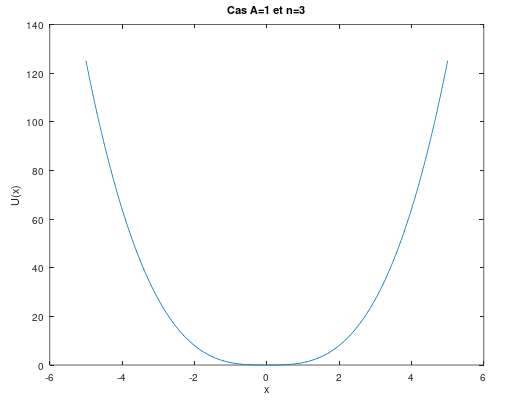
\includegraphics[width=10cm]{chapter_03_exercice_2a}
		\caption{$U = \lvert x \rvert^{n}$ pour $n \in \{1,2,3,4,5\}$}\label{FIG:3_2_a}
	\end{center}
\end{figure}

Dans ce cas pr\'ecis, commen\c{c}ons par d\'efinir les points d'arr\^et tels que $E=U$, soit $x = \pm\left(\dfrac{E}{A}\right)^{\frac{1}{n}}$. Cela permet d'\'ecrire l'\'equation (\ref{EQ:11_5}) telle que :
\bea
	\mathrm{T}(E) & = & \sqrt{2m}\int_{-\left(\frac{E}{A}\right)^{\frac{1}{n}}}^{+\left(\frac{E}{A}\right)^{\frac{1}{n}}}\dfrac{\mathrm{d}x}{\sqrt{E - A\lvert x \rvert^{n}}} \nonumber \\
	& = & 2\sqrt{2m}\int_{0}^{+\left(\frac{E}{A}\right)^{\frac{1}{n}}}\dfrac{\mathrm{d}x}{\sqrt{E - Ax^{n}}} \nonumber \\
	& = & 2\sqrt{\dfrac{2m}{E}}\int_{0}^{+\left(\frac{E}{A}\right)^{\frac{1}{n}}}\dfrac{\mathrm{d}x}{\sqrt{1 - \dfrac{Ax^{n}}{E}}}
\eea
car la fonction $U$ est paire, i.e. $U(x) = U(-x)$. En posant :
\be
	y = \left(\dfrac{A}{E}\right)^{\frac{1}{n}}x
\ee
qui permet d'\'ecrire :
\be
	\begin{cases}
		y^{n} = \dfrac{A}{E}x^{n} \\
		\mathrm{d}y = \left(\dfrac{A}{E}\right)^{\frac{1}{n}}\mathrm{d}x
	\end{cases}
\ee
et :
\be
	\begin{cases}
		x = 0 \Rightarrow y = 0 \\
		x = \left(\dfrac{E}{A}\right)^{\frac{1}{n}} \Rightarrow y = \left(\dfrac{A}{E}\right)^{\frac{1}{n}}\left(\dfrac{E}{A}\right)^{\frac{1}{n}} = 1
	\end{cases}
\ee
La p\'eriode $\mathrm{T}$ devient :
\bea
	\mathrm{T} & = & 2\sqrt{\dfrac{2m}{E}}\int_{0}^{1}\left(\dfrac{E}{A}\right)^{\frac{1}{n}}\dfrac{\mathrm{d}y}{\sqrt{1 - y^{n}}} \nonumber \\
	& = & 2\dfrac{\sqrt{2mE^{\frac{1}{n}-\frac{1}{2}}}}{A^{\frac{1}{n}}}\int_{0}^{1}\dfrac{\mathrm{d}y}{\sqrt{1 - y^{n}}}
\eea
De la m\^eme mani\`ere, en posant $u=y^{n}$, nous avons :
\be
	\begin{cases}
		y = 0 \Rightarrow u = 0 \\
		y = 1 \Rightarrow u = 1
	\end{cases}
\ee
ainsi que :
\be
	\begin{cases}
		y = u^{\frac{1}{n}} \Rightarrow y^{n-1} = u^{\frac{n-1}{n}} = u^{1 - \frac{1}{n}} \\
		ny^{n-1}\mathrm{d}y = \mathrm{d}u \Leftrightarrow \mathrm{d}y = \dfrac{u^{\frac{1}{n} - 1}}{n}\mathrm{d}u
	\end{cases}
\ee
Nous arrivons \`a :
\bea
	\mathrm{T} & = & 2\dfrac{\sqrt{2m}E^{\frac{1}{n}-\frac{1}{2}}}{A^{\frac{1}{n}}}\int_{0}^{1}\dfrac{u^{\frac{1}{n} - 1}\mathrm{d}u}{n(1-u)^{\frac{1}{2}}} \nonumber \\
	& = & 2\dfrac{\sqrt{2m}E^{\frac{1}{n}-\frac{1}{2}}}{nA^{\frac{1}{n}}}\int_{0}^{1}u^{\frac{1}{n} - 1}(1-u)^{\frac{-1}{2}}\mathrm{d}u \label{EQ:APP3_2_a}
\eea
Utilisons ici les int\'egrales d'Euler de premi\`ere esp\`ece, \emph{fonction Béta}, d\'efinies telles que :
\be
	\mathrm{B}(x,y) = \int_{0}^{1}\mathrm{t}^{x-1}(1-\mathrm{t})^{y-1}\mathrm{dt} = \dfrac{\Gamma(x)\Gamma(y)}{\Gamma(x+y)} \label{EQ:INT_EULER_BETA}
\ee
et celles de seconde esp\`ece, \emph{fonction Gamma} :
\be
	\Gamma(z) = \int_{0}^{+\infty}\mathrm{t}^{z-1}e^{-\mathrm{t}}\mathrm{dt} \label{EQ:INT_EULER_GAMMA}
\ee
L'\'equation (\ref{EQ:APP3_2_a}) s'\'ecrit alors :
\bea
	\mathrm{T} & = & 2\dfrac{\sqrt{2m}E^{\frac{1}{n}-\frac{1}{2}}}{nA^{\frac{1}{n}}}\mathrm{B}\left(\frac{1}{n},\frac{1}{2}\right) \nonumber \\
	& = & 2\dfrac{\sqrt{2m}E^{\frac{1}{n}-\frac{1}{2}}}{nA^{\frac{1}{n}}}\dfrac{\Gamma\left(\frac{1}{n}\right)\Gamma\left(\frac{1}{2}\right)}{\Gamma\left(\frac{1}{n}+\frac{1}{2}\right)} \nonumber
\eea
Or $\Gamma(1/2) = \sqrt{\pi}$, nous avons donc finalement :
\be
	\mathrm{T} = 2\dfrac{\sqrt{2\pi m}\Gamma\left(\frac{1}{n}\right)}{nA^{\frac{1}{n}}\Gamma\left(\frac{1}{n}+\frac{1}{2}\right)}E^{\frac{1}{n}-\frac{1}{2}}
\ee

\begin{figure}[htb!]
	\begin{center}
		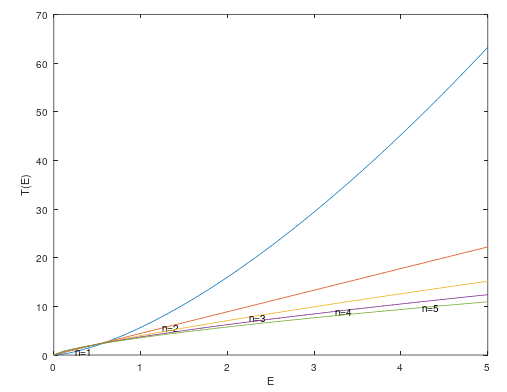
\includegraphics[width=10cm]{chapter_03_exercice_2a_result}
		\caption{$\mathrm{T}(E)$ pour $m=1$, $A=1$ et $n \in \{1,2,3,4,5\}$}\label{FIG:3_2_a_result}
	\end{center}
\end{figure}

\subsubsection{$U = -U_{0}/\cosh^{2}(\alpha x)$ avec $-U_{0} < E < 0$}

\begin{figure}[htb!]
	\begin{center}
		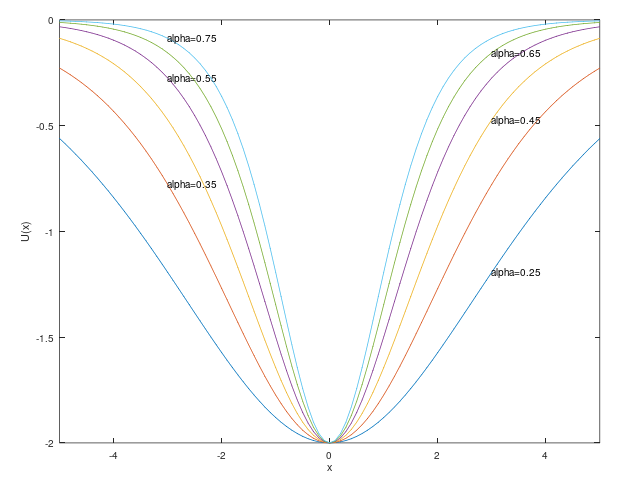
\includegraphics[width=10cm]{chapter_03_exercice_2b}
		\caption{$U = -2 / \cosh^{2}(\alpha x)$ pour $\alpha \in \{0.25,0.35,0.45,0.55,0.65,0.75\}$}\label{FIG:3_2_b}
	\end{center}
\end{figure}

Les point d'arr\^et sont toujours d\'efinis tels que $U=E$, i.e. :
\bea
	\cosh^{2}(\alpha x) & = & -\dfrac{U_{0}}{E} \nonumber \\
	\Leftrightarrow \alpha x & = & \pm \arccosh\left(\sqrt{\dfrac{-U_{0}}{E}}\right)
\eea
Ceci est possible car $-U_{0} < E < 0$ et donc $-U_{0}/E > 0$. Les points d'arr\^et sont donc :
\be
	x = \pm \dfrac{1}{\alpha}\arccosh\left(\sqrt{\dfrac{-U_{0}}{E}}\right)
\ee

L'\'equation (\ref{EQ:11_5}) peut donc s'\'ecrire :
\bea
	\mathrm{T}(E) & = & \sqrt{2m}\int_{-\frac{1}{\alpha}\arccosh\left(\sqrt{\frac{-U_{0}}{E}}\right)}^{\frac{1}{\alpha}\arccosh\left(\sqrt{\frac{-U_{0}}{E}}\right)}\dfrac{\mathrm{d}x}{\sqrt{E + \dfrac{U_{0}}{\cosh^{2}(\alpha x)}}} \nonumber \\
	& = & \sqrt{\dfrac{2m}{\lvert E \rvert}}\int_{-\frac{1}{\alpha}\arccosh\left(\sqrt{\frac{-U_{0}}{E}}\right)}^{\frac{1}{\alpha}\arccosh\left(\sqrt{\frac{-U_{0}}{E}}\right)}\dfrac{\mathrm{d}x}{\sqrt{1 + \dfrac{U_{0}}{E\cosh^{2}(\alpha x)}}}
\eea
car $E < 0$. En choisissant :
\be
	y = \sqrt{\frac{-U_{0}}{E}}\dfrac{1}{\cosh(\alpha x)}
\ee
nous obtenons pour les bornes de l'int\'egrale :
\be
	\begin{cases}
		x = -\frac{1}{\alpha}\arccosh\left(\sqrt{\frac{-U_{0}}{E}}\right) \Rightarrow y = -1 \\
		x = \frac{1}{\alpha}\arccosh\left(\sqrt{\frac{-U_{0}}{E}}\right) \Rightarrow y = 1 \\
	\end{cases}
\ee
et :
\bea
	y^{2} & = & \frac{-U_{0}}{E}\dfrac{1}{\cosh^{2}(\alpha x)} \nonumber \\
	\mathrm{d}y & = & \sqrt{\frac{-U_{0}}{E}}\dfrac{-\alpha}{\cosh^{2}(\alpha x)}\mathrm{d}x \nonumber \\
	\Leftrightarrow & = & -\alpha\sqrt{\frac{-U_{0}}{E}}\dfrac{E}{-U_{0}}y^{2}\mathrm{d}x \nonumber \\
	\Leftrightarrow \mathrm{d}x & = & -\sqrt{\frac{-U_{0}}{E}}\dfrac{\mathrm{d}y}{\alpha y^{2}}
\eea
La p\'eriode s'\'ecrit alors :
\bea
	\mathrm{T}(E) & = & \sqrt{\dfrac{2m}{\lvert E \rvert}}\int_{-1}^{1}\dfrac{y^{-2}\mathrm{d}y}{\sqrt{1-y^{2}}}\times \dfrac{-1}{\alpha}\sqrt{\dfrac{-U_{0}}{E}} \nonumber \\
	& = & -\dfrac{2}{\alpha}\sqrt{\dfrac{-U_{0}}{E}}\sqrt{\dfrac{2m}{\lvert E \rvert}}\int_{0}^{1}\dfrac{y^{-2}\mathrm{d}y}{\sqrt{1-y^{2}}}
\eea

En posant $u = y^{2}$, soit $y = u^{1/2}$ et $\mathrm{d}u = 2y\mathrm{d}y = 2u^{1/2}\mathrm{d}y \Leftrightarrow \mathrm{d}y = \frac{1}{2}u^{-1/2}\mathrm{d}u$, alors la p\'eriode devient :
\bea
	\mathrm{T}(E) & = & -\dfrac{2}{\alpha}\sqrt{\dfrac{-U_{0}}{E}}\sqrt{\dfrac{2m}{\lvert E \rvert}}\int_{0}^{1}\frac{1}{2}\dfrac{u^{-3/2}\mathrm{d}u}{(1-u)^{1/2}} \nonumber \\
	& = & -\dfrac{1}{\alpha}\sqrt{\dfrac{-U_{0}}{E}}\sqrt{\dfrac{2m}{\lvert E \rvert}} \mathrm{B}\left(-\frac{1}{2},\frac{1}{2}\right) \nonumber \\
	& = & \dfrac{2\pi}{\alpha}\sqrt{\dfrac{-U_{0}}{E}}\sqrt{\dfrac{2m}{\lvert E \rvert}}
\eea
car $\Gamma(0) = 1$, $\Gamma(\frac{1}{2}) = \sqrt{\pi}$ et $\Gamma(-\frac{1}{2}) = -2\sqrt{\pi}$. Ici, je trouve une solution diff\'erente de celle propos\'ee par le livre qui est : $\mathrm{T}(E) = \dfrac{\pi}{\alpha}\sqrt{\dfrac{2m}{\lvert E \rvert}}$ et j'avoue ne pas savoir en quoi la p\'riode ne pourrait pas d\'ependre de la profondeur du puits d'\'energie potentielle $U_{0}$.

\subsubsection{$U = U_{0}\tan^{2}(\alpha x)$}

\begin{figure}[htb!]
	\begin{center}
		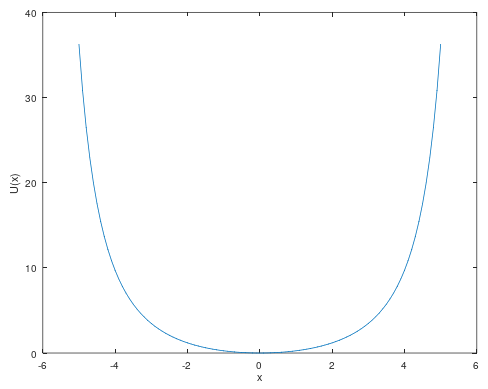
\includegraphics[width=10cm]{chapter_03_exercice_2c}
		\caption{$U = 4\tan^{2}(\alpha x)$ pour $\alpha \in \{0.25,0.35,0.45,0.55,0.65,0.75\}$}\label{FIG:3_2_c}
	\end{center}
\end{figure}

\end{document}
